% =====================================================================
%  AsOfGov -- PVLDB Vol. 20 (2027) research-track submission
%  Assembled main file.  Body target: 12 pages EXCLUDING references.
%
%  TEMPLATE PROVENANCE:
%  acmart.cls (v2.19, 2026/06/27), pvldb.sty (v1.0, 2026/07/06) and
%  ACM-Reference-Format.bst in this directory are verbatim copies from the
%  official template repository github.com/vldbproceedings/VLDB-Template
%  (branch main, retrieved 2026-08-03).  They are vendored next to the
%  source so the build does not silently fall back to whatever acmart
%  version a local TeX Live or Overleaf project happens to ship.
%  Do not edit acmart.cls or pvldb.sty.
% =====================================================================
\documentclass[sigconf, nonacm]{acmart}

%%% do not modify the following VLDB block %%
%%% VLDB block start %%%
\usepackage{pvldb}% VLDB/PVLDB formatting overrides, see pvldb.sty for details.
                      % Do not remove -- required for consistent proceedings
                      % formatting across all VLDB submissions.
%%% VLDB block end %%%

% ---------------------------------------------------------------------
% \artifacturl is the public artifact repository printed in the
% Availability block; \extendedtrurl is the TR's path inside that
% repository.
% ---------------------------------------------------------------------
\newcommand\artifacturl{https://github.com/anon-submit-0/asofgov-artifact}
\newcommand\extendedtrurl{tr/asof-gov-tr.pdf}

% ---- PVLDB issue/paper metadata --------------------------------------
% DOI and page range are assigned during production; placeholders are the
% expected value at submission time (official template README, step 2).
\renewcommand\vldbdoi{XX.XX/XXX.XX}
\renewcommand\vldbpages{XXX-XXX}
\renewcommand\vldbavailabilityurl{\artifacturl}
% pvldb.sty defaults \vldbtitle to \shorttitle, so without this line the
% mandatory PVLDB Reference Format block cites the RUNNING HEAD instead of the
% paper's title.  The optional argument of \title stays the running head (the
% three-line full title would otherwise run as the head on every odd page);
% this macro is what the reference block reads, and it must carry the full
% title with no line break.  Zero page cost -- the block is fixed-height.
\renewcommand\vldbtitle{AsOfGov: As-Of Correctness for Governed Queries with Typed Refusals and Certificates}

\usepackage{amsmath}
\let\Bbbk\relax      % acmart's math font package already defines \Bbbk
\usepackage{amssymb}
\usepackage{booktabs}
\usepackage{multirow}
\usepackage{graphicx}
\usepackage{xcolor}
\usepackage{algorithm}
\usepackage{algpseudocode}
\usepackage{pifont}
\usepackage{balance}

\graphicspath{{figures/}}

% =====================================================================
%  TEMPLATE RESTORATION (2026-08-26).  The route-C typographic-space-
%  recovery block (2026-08-07: microtype protrusion factor 1300, caption
%  skip 4pt, float separations 9pt, booktabs rule padding, \smallskip
%  1pt, theorem surround .25\baselineskip) and the \@BAlancecol
%  ht+dp balancing patch are REMOVED IN FULL: the paper now typesets
%  under acmart/pvldb defaults, nothing but the template's own spacing.
%  The ~25 reclaimed-space debt is paid by content, not glue: the M2
%  abstract + S7.3 compressions and the tab:divergence summary slimming
%  (see sections/08-eval.tex header notes, dated 2026-08-26).
%  The \@BAlancecol patch fixed a balance.sty height-only-accounting bug
%  that produced a 1.1pt overfull \vbox on the references-only page at
%  the 2026-08-07 break position; it is removed WITH the spacing block
%  and is to be re-added (alone, with its documented justification) ONLY
%  if the overfull \vbox resurfaces at the new break position -- the
%  build gate stays 0 errors / 0 overfull / 0 undefined either way.
%  \emergencystretch below is line-breaking, not spacing, and stays.
%
%  2026-08-26, SAME PASS, MEASURED: with the patch removed the template-
%  default build emits exactly one `Overfull \vbox (1.13pt too high) ...
%  while \output is active', shipped from the references-only final page
%  during column balancing -- the documented balance.sty defect (its split
%  loop sizes the two balanced columns by HEIGHT ALONE, then ships each as
%  \vbox to \@tempdima{...\vfil}, so the last line's DEPTH turns into
%  height nobody counted; see the 2026-08-07 \tracingoutput analysis).  The
%  exception foreseen above therefore applies, and the patch below is
%  re-added ALONE: it changes no split point and no content, sizes the two
%  balanced columns by max(ht+dp) instead of max(ht), stays bounded by one
%  real column, and is inert whenever the split lands cleanly.  It is a
%  correctness fix for a package bug, invisible in output -- NOT a spacing
%  override; every route-C item stays removed.
\newsavebox\rcbalcolone
\newsavebox\rcbalcoltwo
\makeatletter
\renewcommand{\@BAlancecol}{\if@twocolumn
  \setbox0=\vbox{\unvbox\@outputbox} \@tempdima=\ht0
  \advance\@tempdima by \topskip \advance\@tempdima
     by -\baselineskip \divide\@tempdima by 2
     \splittopskip=\topskip
  {\vbadness=\@M \loop \global\setbox3=\copy0
   \global\setbox1=\vsplit3 to \@tempdima
   \ifdim\ht3>\@tempdima \global\advance\@tempdima by 1pt \repeat}
   % reassemble both columns exactly as they will be shipped, then measure
   \setbox\rcbalcolone=\vbox{\unvbox1}%
   \setbox\rcbalcoltwo=\vbox{\dimen2=\dp3\unvbox3\kern-\dimen2}%
   % a \vfil follows the unboxed material, so each column's DEPTH turns into
   % height in the box that is actually shipped -- count ht+dp, not ht
   \@tempdimb=\dimexpr\ht\rcbalcolone+\dp\rcbalcolone\relax
   \ifdim\@tempdimb>\@tempdima \@tempdima=\@tempdimb \fi
   \@tempdimb=\dimexpr\ht\rcbalcoltwo+\dp\rcbalcoltwo\relax
   \ifdim\@tempdimb>\@tempdima \@tempdima=\@tempdimb \fi
   \ifdim\@tempdima>\oldvsize \@tempdima=\oldvsize \fi
   \setbox\@leftcolumn=\vbox to \@tempdima{\unvbox\rcbalcolone\vfil}%
   \setbox\@outputbox=\vbox to \@tempdima{\unvbox\rcbalcoltwo\vfil}%
  \fi}
\makeatother
% =====================================================================

% ---------------------------------------------------------------------
%  Line breaking in the identifier-dense and formula-dense passages.
%  Long \texttt{} governance identifiers and long inline math groups are
%  unbreakable boxes; in a 240pt PVLDB column they overshoot the measure
%  and can collide with the neighbouring column.  Two remedies are used,
%  in this order of preference:
%    (1) an explicit \allowbreak after each \_ inside a long identifier
%        (house style, see sections/01-intro.tex) or at a top-level comma
%        of a long inline tuple -- this is the real fix and is applied at
%        every site that produced an overfull box;
%    (2) \emergencystretch as a floor, so that any residual hard case
%        stretches the interword space of its line instead of printing
%        outside the column.  TeX only consults this on the third
%        line-breaking pass, i.e. only for paragraphs that would OTHERWISE
%        produce an overfull box, so paragraphs that already set cleanly
%        are unaffected.  It is a safety net, not a substitute for (1):
%        every site in the 2026-08-03 log was fixed by (1) first, which
%        cut the overfull count from 16 to 6 on its own.
%
%  1.5em was chosen by sweeping 0/1/1.5/2/2.5/3/4em and taking the
%  SMALLEST value that reaches zero overfull \hbox.  It is also the best
%  of the zero-overfull settings on line quality (worst badness 1509,
%  against 2512 at 2em and 2922 at 2.5-3em), and the body page count is
%  identical at every setting.  Do not raise it without re-running that
%  sweep -- at 4em a line hits badness 10000.
% ---------------------------------------------------------------------
\setlength\emergencystretch{1.5em}

% acmart already provides theorem/lemma/proposition/corollary/definition/
% example on a shared section-numbered counter; Sections 3-6 rely on that.

\begin{document}

% The optional short form is the running head; without it the full title runs
% as the head on every odd page and any manual line break inside it propagates
% into \vldbtitle -- so NEVER put \\ in either form.  RETITLED 2026-08-24 to
% the venue-normed form (corpus study of 905 published PVLDB titles: the old
% three-item enumeration subtitle occurs in ~0.2% of titles and was an
% 88th/99th-percentile length outlier; "SystemName: noun-phrase descriptor"
% is the modal pattern at 47%).  The abstract opens "We present
% \textsc{AsOfGov}:", so the system name now leads the title too.  "Binding
% compilation" is the one dropped token -- it is recovered one sentence into
% the abstract.  The tie in "Typed~Refusals" is deliberate: without it the
% two-line page-1 wrap breaks between "Typed" and "Refusals", splitting the
% pair; with it the break falls after "with".
\title[AsOfGov: As-Of Correctness for Governed Queries]{AsOfGov: As-Of
Correctness for Governed Queries with Typed~Refusals and Certificates}

% ---------------------------------------------------------------------
% PVLDB is SINGLE-BLIND: names and affiliations are mandatory on page 1.
% FINAL AUTHOR SET INSTALLED 2026-08-24 (from the author's final
% confirmation, replacing the pre-2026-08-24 single-author placeholder):
% Hongsheng Wang (first author; institutional email replaces the old
% personal the previous personal address; two affiliations, ZJU CS first, Loctek second) and
% Xiubo Liang (corresponding author, marked via \authornote per acmart
% convention).  The PVLDB Reference Format block derives its author list
% from \vldbauthors, which pvldb.sty defaults to acmart's \authors
% accumulator, so both names flow into it with no further edit here.
% \country is mandatory per affiliation (acmart \@ACM@checkaffil raises a
% ClassError without it), so the Loctek affiliation carries its country.
% ---------------------------------------------------------------------
\author{Hongsheng Wang}
\affiliation{%
  \department{College of Computer Science and Technology}
  \institution{Zhejiang University}
  \city{Hangzhou}
  \country{China}
}
\affiliation{%
  \institution{Loctek Ergonomic Technology Corp.}
  \country{China}
}
\email{wanghongsheng@zju.edu.cn}

\author{Xiubo Liang}
\authornote{Xiubo Liang is the corresponding author.}
\affiliation{%
  \department{School of Software Technology}
  \institution{Zhejiang University}
  \city{Hangzhou}
  \country{China}
}
\email{xiubo@zju.edu.cn}

\renewcommand{\shortauthors}{Wang and Liang}

% ABSTRACT COMPRESSED 2026-08-26 (M2 honest-uncertainty pass): the
% elimination accounting now prints the frozen-run verdict beside the
% five-repetition span and the paired nine-cluster CI (gate-wired to
% s3/s4 summary JSONs); the in-abstract frozen-interval straddle and the
% two recoverable-share ceilings moved to S7.3/S9, where they were
% already printed and gated.  Forgery total grew (poststudy3 V6a+).
\begin{abstract}
\looseness=-1 Enterprise analytics increasingly runs through a governed
semantic layer driven by a language model, and the layer moves: calibers are
re-scoped, anchors re-declared, versions advance. Yet
answering a governed question ``as of $T$'' is still treated as a prompting
problem. We show that, under a single-statement,
no-execution-feedback protocol, it is a compile-time \emph{binding} problem.
We present \textsc{AsOfGov}: a bi-temporal governed query semantics whose
typed refusals are values, prove that bindability plus three refusal classes
decidably partition well-formed single-period queries, extend compilation
under a disclosure policy to \textsc{Mlr-Compile} --- a maximal legal
rewrite or a refusal proved complete --- and add point-in-time certificates
checked by
a verifier sharing no module with the compiler. On a fully public 60-question
suite, four frontier model families err on 60.0--76.7\% and
three prompt variants on 53.3--66.7\%. Handed its database's entire
governance layer verbatim, a pre-registered arm still errs on 46.7\%, its
refusal-side errors concentrate where only a data probe decides (6 of 7,
against 1 of 5 on registry-decidable refusals): under this protocol the
frozen run does not cross the pre-registered $40\%$ elimination line (0.361;
five repetitions span 0.361--0.417; paired nine-cluster 95\% CI for absolute
error reduction $[-0.05,0.30]$). The compiler resolves
all 60 questions, a constructive upper bound; the verifier accepts 60 of 60
certificates and rejects 78 of 78 forgeries. Verification costs a paired
median $17.7\times$ the answering query and the certificate
$10.2\times$ the query's bytes.
\end{abstract}

% ---------------------------------------------------------------------
%  CCS concepts and keywords: DECLARED (so they reach the PDF metadata)
%  but NOT PRINTED.  Evidence for not printing them, both checked
%  2026-08-03:
%    (i)  the official Vol.20 template's own main.tex declares neither
%         \ccsdesc nor \keywords;
%    (ii) a published PVLDB paper set from this lineage -- EvoSchema,
%         PVLDB 18(10):3655-3668, vldb.org/pvldb/vol18/p3655-zhang.pdf --
%         prints no "CCS CONCEPTS" and no "KEYWORDS" block on page 1.
%  Printing them cost 0.12 page and put the body OVER the 12-page limit.
%  To restore the printed blocks, delete the \settopmatter line below and
%  reinstate \keywords -- but re-check the page budget first, the body
%  currently ends exactly at the foot of page 12 with no slack.
% ---------------------------------------------------------------------
\settopmatter{printccs=false}
\ccsdesc[500]{Information systems~Query languages}
\ccsdesc[500]{Information systems~Data management systems}
\ccsdesc[300]{Information systems~Temporal data}
\ccsdesc[300]{Computing methodologies~Natural language processing}

\maketitle

%%% do not modify the following VLDB block %%
%%% VLDB block start %%%
\vldbtopmatter
%%% VLDB block end %%%

% =====================================================================
% Section 1 -- INTRODUCTION   (target: ~1.1 page of a 12-page PVLDB body)
% Six-step formula, ONE paragraph per step: background / provenance split
% (production motivation vs public evidence base) / quantified gap /
% concrete example (Fig.1, card_games) / three challenges / "we present" /
% THREE contribution bullets (scope pass AUD-c583a419) + an "Evidence"
% paragraph carrying the headline numbers / positioning.
% EVIDENCE BASE (author ruling, 2026-08-04): every result number in this
% paper is computed on the pilot2 public base (9 BIRD/Spider-lineage
% databases, 60 questions, pilot2/pilot2_summary.json + impl/certs2).
% Enterprise material appears ONLY as motivation and carries an explicit
% production-observation provenance mark.  Do not re-import enterprise
% numbers into any result claim.
% =====================================================================
\providecommand{\sysname}{\textsc{AsOfGov}}
\providecommand{\sem}[1]{[\![#1]\!]}
% Macros needed by the Figure 1 caption; all are \providecommand in
% sections/03-semantics.tex as well.
\providecommand{\ver}{\mathrm{ver}}
\providecommand{\OOV}{\mathsf{OOV}}
\providecommand{\AM}{\mathsf{AM}}
\providecommand{\MC}{\mathsf{MC}}
\providecommand{\ANSW}{\mathsf{ANSWER}}
\providecommand{\REWR}{\mathsf{REWRITE}}
\providecommand{\REFU}{\mathsf{REFUSE}}

\section{INTRODUCTION}
\label{sec:intro}

\looseness=-1 Enterprise analytics is increasingly mediated by a \emph{governed semantic
layer}: metrics, calibers --- the registered conventions fixing which
population a metric attributes over --- and valid-time anchors are
registered as machine-readable objects over the warehouse, so that ``problem
rate'' denotes one agreed computation rather than whatever an analyst
types. Large language models now sit in front of that layer, and the two
interact badly along one axis neither owns: \emph{time}. The layer
moves --- calibers re-scoped, anchors re-declared, versions advancing ---
so a question asked ``as of March'' must be answered under the governance
semantics in force for March, over facts whose valid time falls in March: the
\emph{as-of correctness} problem.

\smallskip\noindent\looseness=-1\textbf{Observed in production, measured in public.}
On the production governance
line behind this work (five governed domains), one problem-rate question
evaluates to a
caliber-aware $16.2\%$ against a caliber-blind $3.8\%$ --- a $4.2\times$ gap
on the same rows. Those are \emph{production observations}: they motivate,
nothing more. Every result number from here
on --- save these rates
and the \S\ref{sec:eval-divergence} ledger, both provenance-marked ---
is computed on a fully public base (nine versioned
BIRD/Spider-lineage databases~\cite{bird,spider}, 3{,}830{,}036 real rows, a
frozen
suite of 60 Chinese questions) whose complete chain ships in the artifact: the
motivation is proprietary, the evidence is not.

\smallskip\noindent\looseness=-1\textbf{The gap is measurable, and one-line prompting does
not close it.} Gold on the 60 Chinese questions is 33 values, 12 governed rewrites and
15 typed refusals (\S\ref{sec:eval}); every arm answers from one statement
without execution feedback, three families behind \S\ref{sec:eval-setup}'s
gateway caveat. Four frontier model families answer 60.0--76.7\%
incorrectly, answering straight through 11, 11, 9 and 13 of the 15
refusals. Three prompt variants of the reference backbone err on
53.3--66.7\%, the best eliminating $22\%$ of its errors against the
pre-registered $40\%$ line (\S\ref{sec:eval-gap}). An arm handing that
backbone its database's \emph{entire} governance layer verbatim still errs on
46.7\% (elimination $36\%$): \emph{under this protocol}, in-context
governance does not substantially close the
gap --- answering through 6
of the 7 probe-decidable refusals and all 3 policy-on-file questions,
correct on 4 of the 5 registry-decidable (\S\ref{sec:eval-gov}).

\smallskip\noindent\looseness=-1\textbf{A running example.} Figure~\ref{fig:running}, from
the public \texttt{card\_games} database, recurs through
\S\ref{sec:semantics}--\S\ref{sec:binding} and is scored in \S\ref{sec:eval}:
in February 2017 \texttt{ruling\_\allowbreak intensity}'s numerator leg is
populated, the same-window denominator empty, the anchor's coverage still
contains February --- no point-in-time correct value exists, and the governed
response is a typed refusal carrying a re-executable witness. Six of the eight
LLM arms answer it anyway, the arm holding the entire governance layer
among them; the
all-history base reports $\approx3.8\%$ (Figure~\ref{fig:running},
bottom row).

% PAGE-BUDGET PASS (B3/B5 merge, 2026-08-03).  This float was fig1_combined.pdf,
% a full-width two-panel figure: (a) the as-of gap, (b) the five-stage pipeline.
% Panel (b) was dropped and the float reverted to the single-column problem
% figure fig1_asof_gap.pdf.  PILOT2 MIGRATION (2026-08-04): the figure is now
% generated from the public card_games warehouse by figures/fig1_asof_gap.py
% (self-contained: queries the warehouse, re-executes the CARD-Q7 witness
% probe, re-tallies the 6/8 from the frozen arm cache; running example
% CARD-Q2/CARD-Q7; the old rma instance survives only as the
% production-observation motivation above).
\begin{figure}[t]
\centering
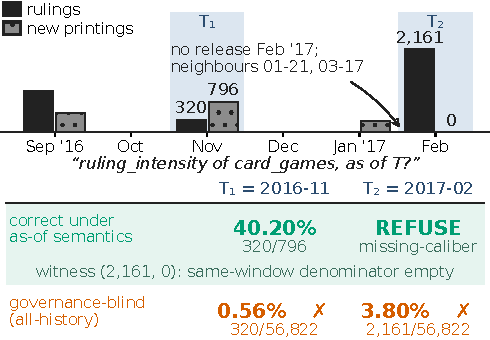
\includegraphics[width=\columnwidth]{fig1_asof_gap.pdf}
\Description{Worked example on the public card games database: the governed
metric ruling intensity at two declared instants. At T1, November 2016, the
compiler answers 40.20 percent; at T2, February 2017, the numerator holds
2,161 rulings but the same-window denominator is empty, so the compiler
issues a typed refusal witnessed by a denominator probe returning zero,
while most evaluated LLM arms answer through.}
\caption{\textbf{The as-of gap.} Under the graph version in effect at the
declared instant ($v_1$ of \texttt{card\_games}; $v_2$ commits 2017-09-28),
\texttt{ruling\_\allowbreak intensity} binds its numerator on
\texttt{rulings.\allowbreak date} and its denominator on
\texttt{sets.\allowbreak releaseDate} under
\texttt{same\_\allowbreak valid\_\allowbreak time\_\allowbreak window}. At
$T_2$ the numerator holds 2{,}161 rulings but the same-window denominator is
empty \emph{inside} validity, so the governed answer is $\bot_{\mathsf{MC}}$,
witnessed by a probe re-evaluating to $0$ (panels and fractions on the
figure).}
\label{fig:running}
\end{figure}

\smallskip\noindent\looseness=-1\textbf{Why this is hard.} Three obstacles organise the technical part.
\emph{(1)~What is the correct answer at a declared time point?} The semantics
must span facts' valid time and the graph's version axis,
and be \emph{total}: refusal is a value it assigns, not an exception raised.
\emph{(2)~Is refusal the last word?} A coarser, masked or narrowed query is
often faithful and legal, so choosing among rewrites needs a fidelity order and
a guarantee that refusal follows an empty legal set, not a search that gave up.
\emph{(3)~Why believe the compiler?} A component that both answers and refuses
is a single point of trust, so the decision must travel with an artifact a
third party re-executes without importing the compiler.

\smallskip\noindent\looseness=-1\textbf{This paper.} We present \sysname, which treats as-of
correctness as a \emph{compile-time binding} problem: a question is bound to a
point on the $\langle$valid-time anchor, governance-graph version$\rangle$
plane, and binding either succeeds or fails in one of three decidable ways.

\begin{itemize}
\item \textbf{A bi-temporal governed query semantics}
  (\S\ref{sec:semantics}): graph versions, valid-time anchors with declared
  coverage modes, and a total point-in-time semantics whose failure values
  $\bot_{\mathsf{OOV}}$, $\bot_{\mathsf{AM}}$, $\bot_{\mathsf{MC}}$ are typed
  refusals; a degeneration theorem exhibits single-version read
  consistency as the two-axis binding's one-dimensional \emph{shape}, at
  construction strength.
\item \textbf{Binding compilation and its decidability}
  (\S\ref{sec:binding}--\S\ref{sec:rewrite}): a coverage theorem partitioning
  well-formed single-period queries into bindable and three disjoint unbindable
  classes, each decidable at a stated cost, the guard order itself part of the
  semantics. Under a disclosure policy it extends to a bounded search,
  \textsc{Mlr-Compile}, proved legal, maximal under deterministic selection,
  complete on refusal.
\item \textbf{Point-in-time certificates and independent verification}
  (\S\ref{sec:certificates}): certificate contents --- anchor assignment,
  version pin, routing path, disclosure decision, witnesses, probe records ---
  and a checking relation decided from graph, data
  and request context alone, with checking completeness, refusal-reason
  soundness
  under the frozen guard order, answer soundness on a template class, and
  per-field non-redundancy.
\end{itemize}

\noindent\looseness=-1\textbf{Evidence} (\S\ref{sec:system}--\S\ref{sec:eval}): a compiler
and a verifier sharing no project-internal module, enforced by a CI import
assertion; nine arms on 60 questions over nine clusters, bootstrap intervals
and coverage beside every rate. The compiler matches the frozen gold
on all 60 (33 answers, 12 rewrites, 15 refusals with reason class), a
\emph{constructive upper bound}; the base exercises the disclosure layer
(3 policy blocks, 5 roll-ups, 2 masks) and the version axis (two committed
versions per database, four value-flipping pairs,
an off-diagonal pin). The verifier accepts $60/60$ certificates,
re-deriving 50 of 60 window coordinates itself (run strictly it fails
closed on the other 10), and rejects $78/78$ forgeries, 44 of them
post-registered after
external review (\S\ref{sec:eval-cert}).
Verifying a decision costs a median
$17.7\times$ the answering query in time and $10.2\times$ in bytes
(\S\ref{sec:eval-cost}). The first cross-check of the two implementations rejected 25 of 51
certificates over 15 root causes (\S\ref{sec:eval-divergence}).

% Measurement marker: start of the theory block (former Section 2 content).
% Theory-block span = page(sec:system) - page(mk:theorystart).  Safe to delete.
\label{mk:theorystart}%
\smallskip\noindent\looseness=-1\textbf{The governed store.} Everything below is stated over
one object: a \emph{versioned governance graph} $G_v$ on an ordinary warehouse
instance $D$, registering metrics, caliber routes, valid-time anchors,
temporal bindings and disclosure policies on an append-only version axis
(\S\ref{sec:semantics}); the nine public databases ship these
tables (847 registry rows), authored by us under three pre-registered
non-degeneracy gates (\S\ref{sec:eval-setup}). Full proofs and omitted
constructions: the extended version~\cite{asofgov-tr}, shipped with the
artifact.

% sections/02-overview.tex is RETIRED (renamed 02-overview.tex.RETIRED,
% 2026-08-06): the governed-store paragraph and the
% roadmap were folded into the end of Section 1, and the pipeline narration
% became panel (b) and the mini-abstract caption of Figure 1 (the merged
% problem+pipeline float emitted from 01-intro; scope pass AUD-c583a419).
% PAGE-BUDGET PASS 2026-08-03: Figure 1 lost panel (b) to fund the cost figure
% (see the comment at the float in sections/01-intro.tex).  The pipeline
% narration therefore now lives ONLY in extended/appendix_proofs.tex and in the
% retired 02-overview.tex; the body has no architecture figure.  This is a
% deliberate, reversible trade, not an oversight.
% =====================================================================
%  Section 3 -- BI-TEMPORAL GOVERNED QUERY SEMANTICS   (source: theory/C3)
%  Needs acmart (+pvldb.sty) and amsmath,amssymb,booktabs,algorithm,
%  algpseudocode.  acmart supplies theorem/lemma/proposition/corollary/
%  definition/example on one section-numbered counter.  Shared macros are
%  defined here (guarded), so this file must be \input before 04/05/06.
%  COMPRESSION: full proofs and the full notation table live in
%  extended/appendix_proofs.tex (extended version, \cite{asofgov-tr}).
% =====================================================================

% ---- shared notation macros (guarded; safe to duplicate in preamble) ----
\providecommand{\Tdom}{\mathbb{T}}
\providecommand{\Qdom}{\mathbb{Q}}
\providecommand{\Wdom}{\mathcal{W}}
\providecommand{\Gfam}{\mathbb{G}}
\providecommand{\Vset}{\mathcal{V}}
\providecommand{\Gseq}{\mathcal{G}}
\providecommand{\Dpol}{\mathcal{D}}
\providecommand{\Mask}{\mathbb{M}}
\providecommand{\ver}{\mathrm{ver}}
\providecommand{\Cov}{\mathrm{Cov}}
\providecommand{\vt}{\mathrm{vt}}
\providecommand{\cmode}{\mathrm{cm}}
\providecommand{\hull}{\mathrm{hull}}
\providecommand{\Pop}{\mathrm{Pop}}
\providecommand{\Bindable}{\mathsf{Bindable}}
\providecommand{\OOV}{\mathsf{OOV}}
\providecommand{\AM}{\mathsf{AM}}
\providecommand{\MC}{\mathsf{MC}}
\providecommand{\DBL}{\mathsf{DB}}
\providecommand{\svw}{\mathrm{svw}}
\providecommand{\legn}{\mathrm{n}}
\providecommand{\legd}{\mathrm{d}}
\providecommand{\ANSW}{\mathsf{ANSWER}}
\providecommand{\REWR}{\mathsf{REWRITE}}
\providecommand{\REFU}{\mathsf{REFUSE}}
\providecommand{\Chk}{\mathsf{Chk}}
\providecommand{\ACC}{\mathsf{ACCEPT}}
\providecommand{\REJ}{\mathsf{REJECT}}
\providecommand{\sem}[1]{[\![#1]\!]}
\providecommand{\dcl}{\mathrm{cl}}
\providecommand{\Legal}{\mathrm{Legal}}
\providecommand{\SUPPMIN}{\mathrm{SUPPMIN}}
\providecommand{\Env}{\mathrm{Env}}
\providecommand{\val}{\mathrm{val}}
\providecommand{\touched}{\mathrm{touched}}
\providecommand{\ctx}{\mathrm{ctx}}
\providecommand{\dec}{\mathrm{dec}}
\providecommand{\out}{\mathrm{out}}
\providecommand{\CT}{\mathrm{CT}}
\providecommand{\srig}{S_{\mathrm{rig}}}
\providecommand{\sraw}{S_{\mathrm{raw}}}
% ------------------------------------------------------------------------

\section{BI-TEMPORAL GOVERNED QUERY SEMANTICS}
\label{sec:semantics}

\noindent\looseness=-1\textbf{Takeaway.}\ \emph{As-of correctness is a property of a
two-axis binding --- the valid-time anchor axis in the data, the version axis
of the governance layer --- and a structured refusal is a first-class value of
it, not an error path.} Proofs are in~\cite{asofgov-tr};
Table~\ref{tab:notation} collects the notation of
\S\ref{sec:semantics}--\S\ref{sec:certificates}.

% =====================================================================
% NOTATION TABLE (added 2026-08-23, review R1-2-2): the body now carries
% the notation of Sections 2-5 itself instead of deferring it to the TR.
% Grouped one line per definition site; the TR keeps the long form.
% =====================================================================
\begin{table}[t]
\centering
\scriptsize
\setlength{\tabcolsep}{2.2pt}
\renewcommand{\arraystretch}{0.93}
\caption{Notation of \S\ref{sec:semantics}--\S\ref{sec:certificates},
in order of definition.}
\label{tab:notation}
\begin{tabular}{@{}ll@{}}
\toprule
$\Tdom$;\ $\Gfam,\sqsubseteq,\sqcap$;\ $\Wdom,\Wdom_g,\top$ &
  time; granularities (refine, meet); windows\\
$a=(o_a,\mathrm{ty}_a,\vt_a,g_a,\cmode_a)$ &
  anchor: object, type, $\vt_a$, granule, mode\\
$V_v(a)$;\ $\Cov_v(a)$ &
  marking set; coverage domain ($\hull$/strict)\\
$G_v=(N_v,E_v,\lambda_v;M_v,R_v,A_v,\beta_v)$ &
  graph at $v$: nodes, edges, labels; registries\\
$M_v$;\ $a_m$ & metric set (atomic/ratio); atomic-metric anchor\\
$R_v(m){=}\rho{=}(\kappa,o_{\mathrm{via}},K_\rho,\mathrm{align}_\rho)$ &
  caliber route: key, via-object, joins, alignment\\
$\beta_v(m)=(a^*_\legn,a^*_\legd,\mathrm{rule})$ &
  temporal binding: leg anchors, rule\\
$\Gseq=(\{G_v\}_{v\in\Vset},\preceq,t)$;\ $\ver(T)$ &
  version sequence, commits; in-effect version\\
$q=(\sigma,T)$;\ $\sigma=(m,s,\vec\omega,\bar a)$ &
  query: intent (metric, scope, $\vec\omega$, $\bar a$), instant\\
$R(q)$;\ $\omega_r$;\ $\uparrow$;\ $\mathrm{RefA}_v$ &
  roles; window map; unresolvable; absent names\\
$\alpha_{q,v}$;\ $P_{\mathrm{rule}}$;\ $\svw$;\ $g^{\mathrm{cmp}}$ &
  candidate asgn.; rule pred.; ref.\ rule; granule\\
$\Pop^{r}_{v,T}(q)$;\ $\mu^{r}_{v,T}(q)$;\ $\models_\rho$ &
  leg population; leg mass; scope match along $\rho$\\
$\Bindable$, (b1)--(b4);\ $\sem{q}_{\Gseq,T}$;\ $\Qdom$ &
  bindability, its guards; semantics; value domain\\
$\bot_{\OOV},\bot_{\AM},\bot_{\MC}$;\ $\DBL$ &
  typed refusals; disclosure-blocked class\\
$\sem{\sigma}^1_{G_v,D}$;\ SVRC;\ (A1)--(A6);\ $n,|W|,|\sem{o}|$ &
  1-axis semantics; consistency; assumptions; costs\\
$\Dpol_v$;\ $L(q,T,\Gseq,\ctx,D)$;\ $X(q,T)$ &
  policies; legal set; candidate space\\
$b=\langle\alpha,w,v,g\rangle$;\ $\dcl(b,\ctx)$;\ $\preceq_D,\approx_D$ &
  binding point; its closure; fidelity order, kernel\\
$\prec_{\det}$;\ $\CT$;\ $U_{\min}$ &
  deterministic key; reason table; legal grains\\
$B=\langle\alpha,\nu,\rho,\delta\rangle$;\ $C=(q,T,B,\out)$ &
  binding quadruple; certificate\\
$\nu$;\ $\delta=(\dec,\Pi,h_{\ctx},g,\mu^*)$;\ $w$ &
  version pin; disclosure decision; refusal witness\\
$\Chk$;\ $\ACC/\REJ$;\ $\mathcal{Q}_{\mathrm{tmpl}}$ &
  checking relation; verdicts; template class\\
\bottomrule
\end{tabular}
\end{table}

\begin{example}[Running example: \textsc{card\_games}]
\label{ex:run}
\looseness=-1 The governed \texttt{card\_games} warehouse registers
\texttt{ruling\_\allowbreak intensity} as a rulings leg over a new-printings
leg, the denominator attributed along the caliber
route \texttt{cards}$\bowtie$\texttt{sets}, both legs bound by
\texttt{same\_\allowbreak valid\_\allowbreak time\_\allowbreak window} over the
day-granular anchors of Figure~\ref{fig:running}. Four requests against that
one registration carry the paper, worked out with every mass in
Figure~\ref{fig:partition}.
\end{example}

\smallskip\noindent\looseness=-1\textbf{Anchors, versions, queries, and the answer
semantics.}\label{sec:sem:graph}\label{sec:sem:bracket}\label{sec:sem:fail}\
\textbf{Time and windows.} $\Tdom$ is a discrete, effectively presented
time domain with decidable order. A
finite granularity family $\Gfam$ (day\dots year) is ordered by refinement
$\sqsubseteq$ and \emph{assumed} a meet-semilattice, $g\sqcap g'$ being the
commonly expressible granularity --- an assumption, not a fact: weeks and months
refine each other in neither direction. The window algebra $\Wdom$ holds
half-open intervals and finite date sets under intersection and containment;
$\Wdom_g$ collects $g$-aligned unions plus $\top$. Request windows are
\emph{capped} to $\bigcup_g\Wdom_g$, so decidability in \S\ref{sec:binding} is
relative to that cap; lifting it to arbitrary definable windows is open.

\noindent\looseness=-1\textbf{Valid-time anchors.} Under version $v$, an anchor is
$a=(o_a,\mathrm{ty}_a,\allowbreak\vt_a,g_a,\cmode_a)$: a semantic object, an
anchor type,
a valid-time assignment $\vt_a:\sem{o_a}_v\to\Wdom$, a marking granularity
$g_a\in\Gfam\cup\{\mathsf{itv}\}$, and a coverage mode
$\cmode_a\in\{\hull,\mathsf{strict\_member}\}$. A \emph{snapshot anchor}
carries an effective date column, $\vt_a(r)=\mathrm{gr}_{g_a}(r.\mathrm{eff})$;
an \emph{interval anchor} ($g_a=\mathsf{itv}$) carries
$(\mathrm{vf},\mathrm{vtc})$ and sets
$\vt_a(r)=[\,r.\mathrm{vf},r.\mathrm{vtc})$ under point-window semantics. The
\emph{marking set} is $V_v(a)=\bigcup_{r\in\sem{o_a}_v}\vt_a(r)$; the
\emph{coverage domain} $\Cov_v(a)$ is $\hull(V_v(a))$ under $\hull$ and
$V_v(a)$ under $\mathsf{strict\_member}$.
Codomain $\Wdom$ admits $\emptyset$: zero-length dimension rows
($\mathrm{vf}=\mathrm{vtc}$) meet every window emptily. Coverage mode is
\emph{per-anchor and versioned}, not global, and every refusal witness
replays it under the declared mode.

\smallskip\noindent\looseness=-1\textbf{Graph versions and the version axis.}
$G_v=(N_v,E_v,\lambda_v;\allowbreak M_v,R_v,A_v,\beta_v)$
(Table~\ref{tab:notation}): layer-labelled nodes, typed edges including
\texttt{numerator\_\allowbreak of}$\langle m\rangle$ and
\texttt{denominator\_\allowbreak of}$\langle m\rangle$; a metric set $M_v$ whose
members are \emph{atomic} $(o_m,f_m)$ or \emph{ratio}
$((o^{\legn}_m,f^{\legn}_m),\allowbreak(o^{\legd}_m,f^{\legd}_m))$; a partial
routing
$R_v(m)=\rho=(\kappa,o_{\mathrm{via}},\allowbreak K_\rho,\mathrm{align}_\rho)$
fixing the \emph{scoped} denominator population; an anchor set
$A_v$, carrying the atomic-metric anchor assignment $m\mapsto a_m$; and a
partial \emph{temporal binding}
$\beta_v(m)=(a^*_{\legn},a^*_{\legd},\mathrm{rule})$, with ``$m$ ratio
$\Rightarrow\beta_v(m)$ defined, each prescribed anchor on its own leg, and a
\emph{distinct}-anchor row declaring a realisation-sensitive clause-(iv)
member'' a well-formedness invariant --- the second clause is what sends
\emph{mixed} coverage to $\AM$(iv) and closes the forward-cited
Theorem~\ref{thm:partition} of \S\ref{sec:binding}.

\noindent\looseness=-1 A \emph{version sequence}
$\Gseq=(\{G_v\}_{v\in\Vset},\preceq,t)$ has $\Vset$ finite non-empty under a
total commit order and a computable strictly monotone commit map
$t:\Vset\to\Tdom$; writing $t_i=t(v_i)$, the \emph{in-effect version} is
$\ver(T)=v_i$ for $T\in[t_i,t_{i+1})$ ($t_{n+1}{=}{+}\infty$), undefined for
$T<t_1$. The axis is \emph{append-only}: committed triples are never
deleted or renumbered, a rollback being a re-commit under a fresh number.

\looseness=-1\emph{Caliber} --- the route $\rho$ fixing over which population a
metric's legs are computed --- \emph{is part of the value, not of
execution.} On the shipped
\texttt{financial} warehouse the same $(m,s,T)$ --- the 1997 penalty-transaction
rate --- evaluates to $0.143\%$ under the registered route (denominator: all
transactions) and to $2.174\%$ under a control route whose denominator is the
penalised-account base itself, a $15.2\times$ gap on the same anchors and
window. Hence the bracket carries $G_v$ as a subscript and $\rho$
must be a certificate field.

\begin{lemma}[version-axis stability]
\label{lem:stability}
\looseness=-1 Let $\Gseq'$ extend $\Gseq$ by appending $v_{n+1}$ with $t_{n+1}>t_n$. Then
$\ver_{\Gseq'}(T)=\ver_{\Gseq}(T)$ and
$\sem{q}_{\Gseq',T}=\sem{q}_{\Gseq,T}$ for every $T<t_{n+1}$ and every $q$
declared at $T$.
\end{lemma}

\noindent\looseness=-1 Proof in~\cite{asofgov-tr}. Point-in-time answers, refusals included,
are durable assertions about $(T,v)$. \emph{In our seeds}, four
question pairs flip value under the version change alone
(\S\ref{sec:eval}).

\begin{definition}[bi-temporal query and candidate assignment]
\label{def:query}\label{def:alpha}
\looseness=-1 A query is $q=(\sigma,T)$ with declared instant $T$ and structured intent
$\sigma=(m,s,\vec\omega,\bar a)$.
\par\noindent\textbf{(1)~Intent.} $m$ is a metric reference and $s$ a scope
selector; $\vec\omega$ assigns each role
$r\in R(q)\subseteq\{\mathrm{num},\mathrm{den},\mathrm{atom}\}$ a computable
\emph{window derivation} $\omega_r:\Tdom\to\Wdom\uplus\{\uparrow\}$ with an
explicit unresolvable sentinel; $\bar a$ is a partial \emph{anchor override}
from roles to anchor \emph{references by name}, not presumed to resolve in
$A_v$.
\par\noindent\textbf{(2)~Candidate assignment.} For $v=\ver(T)$
and $m\in M_v$, with $\mathrm{RefA}_v$ the override names failing to resolve
in $A_v$, the candidate assignment is the \emph{function}
$\alpha_{q,v}:R(q)\rightharpoonup(A_v\uplus\mathrm{RefA}_v)\times\Wdom$,
$\alpha_{q,v}(r)=(\bar a(r)\text{ else prescribed},\ \omega_r(T))$, the
prescribed anchors being the two legs of $\beta_v(m)$ (ratio) or $a_m$
(atomic).
\par\noindent\textbf{(3)~Unresolved overrides.} An override resolving into
$\mathrm{RefA}_v$ keeps the role out of the $\OOV$ coverage disjunct and
classifies the query $\bot_{\AM}$, witness ``declared name absent from
$A_v$'', for ratio and atomic metrics alike (once $\neg\OOV$;
Definition~\ref{def:am}(2), a forward reference).
\end{definition}

\looseness=-1 That $\alpha_{q,v}$ is a function --- no search --- is deliberate: the
existential quantifier over assignments is \S\ref{sec:rewrite}'s. The
definitions sit on the \emph{diagonal} $T_{\mathrm{vt}}=T_{\mathrm{ver}}=T$;
our suite runs the two-parameter bracket ($T_{\mathrm{ver}}$ declaring,
$T_{\mathrm{vt}}$ as-of), carried statement by statement
in~\cite{asofgov-tr}; admissibility stays a disclosure question.

\begin{definition}[binding rule; \texttt{same\_valid\_time\_window}]
\label{def:rule}
\looseness=-1 Each rule denotes a decidable $P_{\mathrm{rule}}(\alpha;G_v,D)$. The reference
rule $\svw$ holds on
$\alpha=\{\mathrm{num}\mapsto(a_\legn,W_\legn),\mathrm{den}\mapsto(a_\legd,W_\legd)\}$
when all four clauses hold:
\par\noindent\textbf{(i) anchor fidelity:}
$a_\legn=a^*_\legn,a_\legd=a^*_\legd$;
\par\noindent\textbf{(ii) same window:} $W_\legn=W_\legd=:W$;
\par\noindent\textbf{(iii) window--granularity expressibility:}
$W\in\Wdom_{g^{\mathrm{cmp}}}$ for the declared comparison granularity, by
default $g_{a^*_\legn}\sqcap g_{a^*_\legd}$ over the legs whose $g_a$ lies in
$\Gfam$ (an interval-anchored leg imposes no granule constraint; where neither
leg has one, $g^{\mathrm{cmp}}$ must be declared);
\par\noindent\textbf{(iv) anchor-pair admissibility:} a member of a finite
decidable check library fixed by the binding row's anchor pair --- trivially
true, or a symmetric-difference audit on the marking domains or on the
window-restricted realisations.
\end{definition}

\looseness=-1 Clause~(iv) reaches into governance content: the check
library is versioned data, not part of the abstraction (its teeth:
Example~\ref{ex:symdiff}).

\begin{definition}[bindability]
\label{def:bindable}
\looseness=-1 With $v=\ver(T)$, $\rho=R_v(m)$ and $\alpha_{q,v}(r)=(a_r,W_r)$, the leg
population and mass are
$\Pop^{r}_{v,T}(q)=\{x\in\sem{o^{r}_m}_v: x\models_\rho s,\allowbreak\
\vt_{a_r}(x)\cap W_r\neq\emptyset\}$ and
$\mu^{r}_{v,T}(q)=\sum_{x\in\Pop^{r}_{v,T}(q)}f^{r}_m(x)$, where
$x\models_\rho s$ means $x$ matches the scope after transfer along the route's
join keys and attribution alignment. $\Bindable(q,\Gseq,D)$ holds when:
\par\noindent\textbf{(b1)} \emph{both axes in effect} --- $\ver(T)$ defined,
each $\omega_r(T)$ defined, and per role $a_r\in A_v$ with
$W_r\cap\Cov_v(a_r)\neq\emptyset$;
\par\noindent\textbf{(b2)} \emph{metric, route and binding registered} ---
$m\in M_v$, and for a ratio $R_v(m)$ defined and recomputable and
$\beta_v(m)$ defined;
\par\noindent\textbf{(b3)} \emph{rule satisfied} ---
$P_{\mathrm{rule}}(\alpha_{q,v};G_v,D)$ whenever $\beta_v(m)$ is defined;
\par\noindent\textbf{(b4)} \emph{positive denominator mass} ---
$\mu^{\mathrm{den}}_{v,T}(q)>0$ for a ratio.
\end{definition}

The legs are asymmetric: a zero numerator mass is a lawful $0$ where a zero
denominator mass destroys the ratio.

\begin{definition}[point-in-time answer semantics]
\label{def:bracket}
\looseness=-1 The denotation is the \emph{total} function $\sem{q}_{\Gseq,T}:
\text{queries}\to\Qdom\cup\{\bot_{\OOV},\bot_{\AM},\bot_{\MC}\}$ given by
$\mu^{\mathrm{num}}_{v,T}(q)/\mu^{\mathrm{den}}_{v,T}(q)$ if $\Bindable$ and
$m$ is a ratio, $\mu^{\mathrm{atom}}_{v,T}(q)$ if $\Bindable$ and $m$ is
atomic, and otherwise $\bot_c$ for the first failing guard $c$. Numerator and
denominator are bound separately to the valid-time window of $T$ through their
own anchors, and jointly to the version $\ver(T)$ in effect at $T$: this is
the two-dimensional binding. Delta and multi-period intents expand by role
$\times$ period and resolve lexicographically
(Corollary~\ref{cor:multi}, a forward
reference), keeping $\sem{\cdot}$ single-valued.
\end{definition}

\begin{proposition}[well-definedness]
\label{prop:welldef}
\looseness=-1 When $\Bindable(q,\Gseq,D)$ holds, $\sem{q}_{\Gseq,T}$ is determined by
$(q,\Gseq,D)$ and independent of evaluation order.
\end{proposition}

\noindent\looseness=-1 Proof in~\cite{asofgov-tr}. \emph{Ratio-of-sums invariant:} each leg is
aggregated over the window before dividing, since for $W=\biguplus_j W_j$
$\sum_j\mu^{\legn}_j/\sum_j\mu^{\legd}_j$ and the average of per-part ratios
differ; the template's \texttt{sum(rate)} ban and the verifier's ratio-shape
check are its two projections.

\begin{definition}[the three refusal classes, as a guard chain]
\label{def:oov}\label{def:am}\label{def:mc}
\looseness=-1 Each predicate is defined under the negation of its predecessors, which makes
them pairwise disjoint and keeps every object they mention nameable.
\textbf{(1) $\OOV$ (out-of-validity)}: $\ver(T)$ undefined, or some
$\omega_r(T)=\uparrow$, or coverage vacuity over the single-period roles
--- \emph{pair-level} where $\beta_v(m)$'s rule pairs two legs (both
realisations empty; mixed is Definition~\ref{def:rule}(iv)'s audit
jurisdiction), per-role $W_r\cap\Cov_v(a_r)=\emptyset$ for an unpaired
(atom) role --- the reading frozen before any model call (deviation ledger
\texttt{PORT\_REPORT} \S4(2), in the artifact). A disjunct naming a non-nameable object
counts as false, so a missing object cannot masquerade as temporal failure.
\textbf{(2) $\AM$ (anchor-mismatch), guarded by $\neg\OOV$}: $\beta_v(m)$
defined and $\neg P_{\mathrm{rule}}(\alpha_{q,v};G_v,D)$, witnessed by
whichever clause of Definition~\ref{def:rule} fails; or some declared
override resolves into $\mathrm{RefA}_v$ --- witnessed by the name absent
from $A_v$, the $\AM$(i) form --- for ratio and atomic metrics alike.
\textbf{(3) $\MC$ (missing-caliber), guarded by $\neg\OOV\wedge\neg\AM$}:
\emph{(i)} $m\notin M_v$, or $m$ a ratio with $R_v(m)$ undefined or not
recomputable or $\beta_v(m)$ undefined; or \emph{(ii)} $m$ a ratio with
$\mu^{\mathrm{den}}_{v,T}(q)\le0$.
\end{definition}

\looseness=-1 The $\OOV$/$\MC$(ii) boundary is the paper's most consequential
adjudication: $\OOV$ carries \emph{coverage vacuity} --- the window missing
the coverage domain altogether --- whereas zero denominator mass
\emph{inside} that domain is a caliber failure (Figure~\ref{fig:partition}
exhibits both on one scope); widening $\MC$(ii) to $\mu_{\mathrm{den}}\le0$
also covers refund-reversal populations --- non-empty, non-positive mass ---
a regime the \S\ref{sec:rewrite} guarantees exclude
(Theorem~\ref{thm:refusal}). The scope selector
$s$ is a predicate, not a governed object --- a scope matching nothing is
lawful ($0$ atomic, $\MC$(ii) ratio) --- a membership guard is future work.

\smallskip\noindent\looseness=-1\textbf{Degeneration: the one-dimensional shadow.}%
\label{sec:sem:degen}
Fix $(G_v,D)$. The \emph{single-version} semantics $\sem{\sigma}^1_{G_v,D}$
drops anchor--window filtering but retains the anchor-validity restriction
$\vt_{a_r}(x)\neq\emptyset$; an evaluation satisfies
\emph{single-version read consistency} (SVRC) iff a single committed
version $v$ supplies every governance object it reads --- metric record,
route, anchors, binding row --- and the one snapshot $D$ every fact ---
a definition complete here (restated in~\cite{asofgov-tr}).

\begin{theorem}[degeneration]
\label{thm:degen}
\looseness=-1 Let $\mathcal{Q}^{\downarrow}$ be the queries satisfying \textbf{(H1)}
$T\ge t_n$, hence $\ver(T)=v_n$; \textbf{(H2)} $\omega_r(T)=\top$ for every
role; \textbf{(H3)} $\bar a=\emptyset$. Then for every
$q\in\mathcal{Q}^{\downarrow}$: \emph{(1)} the evaluation satisfies SVRC,
witnessed by $v_n$; \emph{(2)} whenever $\sem{q}_{\Gseq,T}\in\Qdom$ it equals
$\sem{\sigma}^1_{G_{v_n},D}$; \emph{(3)} each failure class collapses to a
non-temporal residue --- $\AM$ to a failure of clause~(iv) alone, $\OOV$ to
$V_{v_n}(a)=\emptyset$ for every prescribed anchor, and $\MC$ to a missing route
or a non-positive domain-wide scoped denominator mass.
\end{theorem}

\noindent\looseness=-1 Proof in~\cite{asofgov-tr}. Every $\Bindable$ evaluation satisfies
SVRC, witnessed by $\ver(T)$; under (H1)--(H3) the temporal content collapses
entirely to it. \emph{Honest strength:} under the snapshot assumption clause~(1) holds \emph{by
construction}; re-proving a concurrency guarantee under version advance needs
a per-datum read-version function a single-snapshot $D$ cannot express --- the
shape of a substrate guarantee at construction strength, not its
subsumption.

% =====================================================================
%  Section 4 -- BINDING COMPILATION            (source: theory/C3 §5)
%  Requires macros defined in 03-semantics.tex (\input that file first).
%  Full proofs: extended/appendix_proofs.tex (\cite{asofgov-tr}).
% =====================================================================

\section{BINDING COMPILATION}
\label{sec:binding}

\noindent\looseness=-1\textbf{Standing assumptions} for this section and the next:
\textbf{(A1)} each extension $\sem{o}_v\subseteq D$ is finite and enumerable
with bounded per-fact predicate cost; \textbf{(A2)} valid-time assignments and
window operations are computable and $\Gfam$ is a finite meet-semilattice with
day as common refinement; \textbf{(A3)} $\Vset$ is a non-empty finite total
order, the commit map is computable and strictly monotone, and the version axis
is append-only; \textbf{(A4)} every rule in the library denotes a decidable
predicate; \textbf{(A5)} each window derivation is a total function into
$\Wdom\uplus\{\uparrow\}$, so ``$\omega_r(T)$ unresolvable'' is one evaluation
and not a halting question; \textbf{(A6)} $\Tdom$ is discrete, effectively
presented, with decidable order --- continuous time domains, where endpoint
comparison is only semi-decidable, are out of scope.

\label{sec:bind:partition}%
\begin{theorem}[coverage partition, single period]
\label{thm:partition}
For every well-formed single-period query $q$ --- $\sigma$ syntactically well
formed, $T\in\Tdom$, and $R(q)\subseteq\{\mathrm{num},\mathrm{den}\}$ or
$R(q)=\{\mathrm{atom}\}$ --- under \emph{(A1)--(A6)} the four cases
\textbf{(a)} $\Bindable$, \textbf{(b)} $\OOV$, \textbf{(c)}
$\neg\OOV\wedge\AM$, \textbf{(d)} $\neg\OOV\wedge\neg\AM\wedge\MC$ are
pairwise disjoint and jointly exhaustive, and
$\sem{q}_{\Gseq,T}\in\Qdom\iff$(a), $=\bot_{\OOV}\iff$(b),
$=\bot_{\AM}\iff$(c), $=\bot_{\MC}\iff$(d).
\end{theorem}

\noindent\looseness=-1 Proof in~\cite{asofgov-tr}: disjointness follows from the guard
chain and obligations (b1)--(b4) of Definition~\ref{def:bindable};
exhaustiveness uses Proposition~\ref{prop:decidable}, whose proof does not use
this theorem, to make each guard two-valued on its domain, and the
vacuity convention of Definition~\ref{def:oov} to keep a missing object out of
the temporal door. Figure~\ref{fig:partition} walks one request into
each of the four outcomes on a single store.
% The four-case walk that used to be prose here is Figure~\ref{fig:partition},
% which prints every mass; keep this pointer, not a second telling of it.

% Emitted at exactly \columnwidth by figures/figA_partition.py -- include at
% natural size; the 5.4 pt type floor is stated for that placement and does not
% survive a down-scale.  Data: figures/fig_data_p2.json["partition"], recomputed
% from the public card_games warehouse and cross-asserted against impl/certs2/.
\begin{figure}[t]
\centering
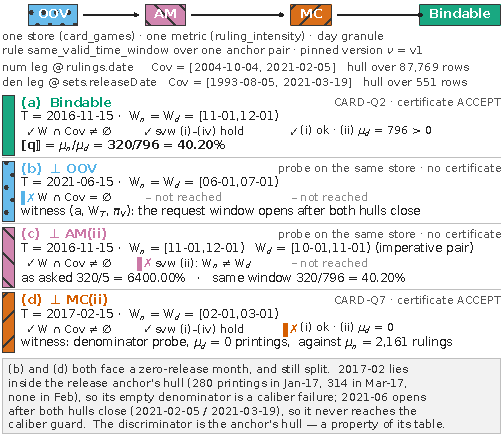
\includegraphics[width=\columnwidth]{figA_partition.pdf}
\Description{Four sibling requests on the same governed metric walked
through the guard chain in its frozen order, one row per request: each row
prints the request window, the outcome of every guard with the quantity
that decided it, and the exit --- one bound answer and the three refusal
classes --- so the four rows realise the four-way partition while only the
window coordinates differ.}
\caption{The partition on four sibling requests to the \texttt{card\_games}
store: only the coordinates move, so each row leaves the chain in a different
column. (b) and (d) are the $\OOV$/$\MC$(ii) boundary --- one metric, one
empty same-month denominator, two classes --- because $\Cov$ is the hull of
the \emph{anchor's} table: 2017-02 lies inside it, 2021-06 after it. (c)~is
what a refusal buys: the $6400\%$ its cross-window binding would report
against the $40.2\%$ the same-window rule delivers in (a). (a) and (d) are
suite questions with verifier-accepted certificates; (b) and (c) are probes on
the same store, and say so.}
\label{fig:partition}
\end{figure}

\smallskip\noindent\textbf{Decidability, cost, multiple periods, and guard
order.}\label{sec:bind:decidable}
\nopagebreak

\begin{proposition}[decidability and cost]
\label{prop:decidable}
\looseness=-1 Under \emph{(A1)--(A6)}, $\OOV$, and $\AM$ and $\MC$ on their guard domains,
are decidable by constructive procedures at the following costs ($n=|\Vset|$,
$|W|$ the window description length, $|\sem{o}|$ extension cardinality).
\textbf{$\OOV$:} locate $\ver(T)$ by binary search over $t_1<\cdots<t_n$;
evaluate $\omega_r(T)$ through its total presentation, sentinel included;
compute coverage by the declared mode --- one scan taking $\min/\max$ for
$\hull$, a sort-and-merge into an interval union for
$\mathsf{strict\_member}$, zero-length rows skipped --- and intersect with the
normal form of $W_r$; cost
$O(\log n)+\sum_r O(|\sem{o_{a_r}}|\log|\sem{o_{a_r}}|+|W_r|)$.
\textbf{$\AM$:} clause~(i) is an identifier comparison, (ii) a normal-form
equality, (iii) a granule-boundary alignment test on each maximal interval of
$W$, and (iv) a call into the declared check library --- constant for the
trivial variant, one scan over both anchor objects for the
symmetric-difference audit, windowed for the realisation variant; cost
$O(|W|\log|W|)+O(|\sem{o_{a^*_\legn}}|+|\sem{o_{a^*_\legd}}|)$.
\textbf{$\MC$:} mode~(i) is a key lookup in $M_v,R_v$, mode~(ii) one scan over
$\sem{o^{\legd}_m}_v$ accumulating $f^{\legd}_m$; cost
$O(|\sem{o^{\legd}_m}|)$.
\end{proposition}

\noindent\looseness=-1 Proof in~\cite{asofgov-tr}; (A5) is where it would break: from
partial computability alone, deciding $\omega_r(T)=\uparrow$ is a halting
question. Each procedure also emits, as a by-product, the failing
clause or the probe with its asserted result --- the witness content
\S\ref{sec:certificates} requires: decision procedure and witness
generator are one object seen twice.

\begin{example}[clause~(iv) with teeth]
\label{ex:symdiff}
\looseness=-1\texttt{EF2-Q6} asks the rating-weighted daily win rate of
\texttt{european\_\allowbreak football\_2} as of 2013-12-01: the numerator
leg binds to the match-day anchor under hull coverage, the denominator leg
to the rating-snapshot anchor, a date-set anchor under
$\mathsf{strict\_member}$ whose weekly marking dates surround the day
(2013-11-29, 2013-12-06) without containing it. The discriminant is
clause~(iv), the window-realisation audit this pair prescribes: on the
single-day window the match anchor realises 33 rows, the snapshot anchor
none, differing on exactly one date; the certificate carries 2013-12-01
with both counts, recounted by the verifier from $D$. A check on the
rule \emph{literal} alone would accept (\S\ref{sec:rewrite}): the same seed binds
\texttt{win\_\allowbreak rate} under that literal with both legs on one
anchor.
\end{example}

\begin{corollary}[per-period classification]
\label{cor:multi}
\looseness=-1 A delta or multi-period query expands by role $\times$ period into a finite
family $\{q^{(j)}\}_j$ of single-period queries in the declared period order.
Theorem~\ref{thm:partition} applies to each $q^{(j)}$, and the value of the
whole query is lexicographic: if every $q^{(j)}$ falls in case~(a),
$\sem{q}_{\Gseq,T}$ is the declared arithmetic combination of the per-period
values; otherwise it is $\sem{q^{(j_0)}}_{\Gseq,T}$ for the first failing
period $j_0$. Two side conditions make this well posed: guard predicates and
$P_{\svw}$ are evaluated on the single-period restriction
$\alpha_{q,v}|_{R(q^{(j)})}$, and the existential quantifier over roles inside
$\OOV$ does not range across periods.
\end{corollary}

\looseness=-1 The second condition is forced by an instance: the delta over
$[\,2017\text{-}02,$\linebreak[0] $2021\text{-}06\,]$ on
Figure~\ref{fig:partition}'s store (b,\,d) has periods $\bot_{\MC}$ and
$\OOV$; a cross-period quantifier would report $\bot_{\OOV}$, the
lexicographic rule $\bot_{\MC}$.

\smallskip\noindent\looseness=-1\textbf{Guard order is not cosmetic.}%
\label{sec:bind:guardorder}
The three raw conditions can hold at once; the chain resolves the class to the
first. Example~\ref{ex:symdiff} is the suite's live
collision: on the single-day window the snapshot leg's
$\mathsf{strict\_member}$ coverage is empty, so a leg-at-a-time $\OOV$
reading fires before the audit and returns $\bot_{\OOV}$ --- same
witness replay, wrong reason class.
Definition~\ref{def:oov}(1)'s pair-level clause rules that out --- the
realisation is mixed --- and gold is
$\bot_{\AM}$(iv). Adjudications of this kind, left unregistered, are what
\S\ref{sec:eval-divergence} measures. We report no permutation ablation over
the six guard orders.

% =====================================================================
%  Section 4 -- DISCLOSURE-CONSTRAINED REWRITING     (source: theory/C4)
%  SCOPE DECISION (audit AUD-c583a419, scope pass): the MLR development was
%  demoted from a headline contribution to a compact section.  The body
%  KEEPS the one-paragraph policy model, the MLR problem definition, the
%  three statements (soundness / maximality / determinism and refusal
%  completeness) with their original labels -- \S\ref{sec:certificates} and
%  \S\ref{sec:eval} cite them -- and the interface sentence to the guard
%  order OOV -> AM -> MC.  MOVED to extended/appendix_proofs.tex
%  (\cite{asofgov-tr}): Algorithm 1 and its line-level commentary, the grain
%  and mask lattice machinery, the (S-A)..(S-M) coordinate semantics, the
%  monotonicity and grain-frontier lemmas, the pruning corollary, and the
%  complexity theorem with its proof.
%
%  PAGE-BUDGET PASS (B3/B5 float funding, 2026-08-03).  This section was the
%  plan's designated donor when the layer had ZERO instances on the old
%  51-question development suite.  Externalised to the TR in that pass: the
%  elaborated mask derivation (mu*, top_Mask, the empty-shell argument), the
%  binding-point range commentary, the frontier construction, and the two
%  proof sketches.  DELETED as duplication rather than moved: the
%  instance/context-relativity justification and the ungoverned-disclosure
%  annotation gloss, both already carried by \S\ref{sec:cert:content}.
%  PILOT2 MIGRATION (2026-08-04): on the public base the layer IS exercised
%  (3 DISCLOSURE-BLOCKED + 5 roll-ups + 2 masks in gold; 10 F4 forgeries),
%  so the "unexercised here" honesty sentence became the exercised-scope
%  sentence -- do not resurrect the old wording.
%  RED LINES kept verbatim: Theorem~\ref{thm:sound}/\ref{thm:maximal} and
%  Theorem~\ref{thm:refusal} statements with their assumption recitals; the
%  full-rule-predicate guard with Example~\ref{ex:symdiff}'s discriminant;
%  the three open boundaries.
%  Requires macros from 03-semantics.tex.
% =====================================================================

\section{DISCLOSURE-CONSTRAINED REWRITING}
\label{sec:rewrite}

\noindent\looseness=-1 Under a disclosure policy, binding compilation extends from a decision
to a bounded search over binding points, with refusal a proof that the legal set
is empty rather than an abstention. The search runs \emph{after} the guard order
$\OOV\rightarrow\AM\rightarrow\MC$ has been discharged on a slice and $\DBL$
follows all three, so a legally trimmed answer never becomes an answer to a
different question at a different time point.

\smallskip\noindent\looseness=-1\textbf{The policy model, MLR, and the compiler.} $G_v$
declares a finite grain lattice whose roll-up edges are registered and never
inferred from data, a finite mask lattice, and a finite versioned set $\Dpol_v$
of \emph{disclosure policies}, each pairing a protected attribute set with a
role branch, a minimum mask, a grain floor and a small-cell threshold; a
candidate is \emph{admissible} when every policy whose protected closure it
touches is discharged by one of those branches. The \emph{legal set}
$L(q,T,\Gseq,\ctx,D)$ collects the closures of the \emph{binding points}
$b=\langle\alpha,w,v,g\rangle$ of the \emph{structural} candidate space
$X(q,T)$ of~\cite{asofgov-tr} --- one window candidate per slice, no
data-driven shrinking --- faithful to the question's rigid
commitments, bindable (Definition~\ref{def:bindable}) and admissible; one masking
a rigidly requested attribute away entirely is refused
\emph{disclosure-blocked} ($\DBL$), not answered with an empty shell.
\textbf{MLR} (\emph{maximal legal rewrite}) asks for either $\ANSW$ from a
$\preceq_D$-maximal element of
$L/\!\approx_D$ under the \emph{fidelity order} $\preceq_D$ --- which compares
only same-anchor, same-version points, $b\preceq_D b'$ when $b'$ trims no more
of the window at no coarser a grain, $\approx_D$ its symmetric kernel ---
or $\REFU$ with a
per-slice reason table $\CT$ over $\{\MC,\AM,\OOV,\DBL\}$ evidencing
$L=\emptyset$; \textsc{Mlr-Compile} solves it slice by slice under a declared
total order; the algorithm, the lattices' coordinates, the frontier and
pruning lemmas and a polynomial probe bound are in~\cite{asofgov-tr}. One guard
must be named because both statements below rest on it: the rule test
evaluates the \emph{full} predicate of Definition~\ref{def:rule}, clauses
(i)--(iv), not the rule literal --- the binding row of
Example~\ref{ex:symdiff} carries the same
\texttt{same\_\allowbreak valid\_\allowbreak time\_\allowbreak window} literal
as its trivially compatible siblings, and a literal-only check answers the
request its audit refuses.
\emph{Scope:} four of the nine domains register policies (18 instance rows),
the other five carrying the
\texttt{ungoverned-disclosure} annotation of \S\ref{sec:cert:content}. The suite binds the layer our
development seeds only formalised: 3 questions refuse \textsc{disclosure-blocked} on a replayed
small-cell probe, 5 answer only after a granularity roll-up --- one under a
threshold the version change raises --- and 2 only under a mask closure
(\S\ref{sec:eval-mech}); 10 of the 34 forgeries attack this layer.

\begin{theorem}[soundness, maximality, determinism]
\label{thm:sound}\label{thm:maximal}
\looseness=-1 Assume \emph{(A1)--(A6)} of \S\ref{sec:binding} together with: the declared
lattices are finite and the grain lattice's roll-up edges are registered;
$\Dpol_v$ is finite and every policy is coarsening-compatible;
$\prec_{\det}$ is a total key over versioned components of $G_v$; and
\emph{(A-emit)}: the code emitter is point-in-time correct on bindable
closures --- the syntax-to-semantics bridge assumed as A4.1 in~\cite{asofgov-tr}
and recorded open there (gap G2), an obligation of the same kind as
Theorem~\ref{thm:certsound}(b)'s declared scope.
\emph{(a)} If \textsc{Mlr-Compile} returns $\ANSW$ then
$\dcl(\hat b,\ctx)\in L(q,T,\Gseq,\ctx,D)$ and the emitted plan is
point-in-time correct in the sense of Definition~\ref{def:bracket}.
\emph{(b)} Every element of the frontier is $\preceq_D$-maximal in
$L/\!\approx_D$, and the returned $\hat b$ is one of them.
\emph{(c)} The returned representative is a function of
$\langle q,T,\Gseq,\Dpol,\ctx,D\rangle$, since all three keys of
$\prec_{\det}$ are versioned components of $G_v$; re-declaring $\prec_{\det}$
changes the representative, not the maximal set and not the $\ANSW$/$\REFU$
verdict.
\end{theorem}

\begin{theorem}[refusal completeness]
\label{thm:refusal}
\looseness=-1 Under the same assumptions, and with the denominator measure non-negative,
\textsc{Mlr-Compile} returns $\REFU$ iff $L(q,T,\Gseq,\ctx,D)=\emptyset$. On
refusal, $\CT$ carries a per-slice emptiness witness whose reasons decompose
into the three binding-layer classes of \S\ref{sec:sem:fail} plus the
disclosure-layer class $\DBL$; when $\Dpol_v=\emptyset$, $\DBL$ is unreachable
and the statement reduces to binding completeness.
\end{theorem}

\noindent\looseness=-1 Both proofs are in~\cite{asofgov-tr}; refusal completeness is
precisely where the full rule predicate is required.
\textbf{Boundaries.} Three stay open: window bargaining needs
a joint window--grain maximality theory (both theorems above are relative to
$X$); we return one maximal element per slice
frontier and do not bound the cost of enumerating all of them; and the rule
language is confined to window-equality rules, so lag bindings need an extended
predicate. Theorem~\ref{thm:refusal}'s stated premise, like the probe
bound, assumes a non-negative denominator measure --- with
refund-reversal columns the mass is not monotone along window containment and
the pruning argument fails.

% =====================================================================
%  Section 6 -- POINT-IN-TIME CERTIFICATES     (source: theory/C5)
%  Requires macros from 03-semantics.tex; booktabs in the preamble.
%  Full proofs: extended/appendix_proofs.tex (\cite{asofgov-tr}).
% =====================================================================

\section{POINT-IN-TIME CERTIFICATES}
\label{sec:certificates}

\noindent\looseness=-1 Compilation and verification read the
same $(G_v,D)$ snapshot, and two commit axioms --- typed commit identifiers
unique and fresh, version numbers never reused --- keep a certificate valid
\emph{at its coordinate} $(T,v)$.

\subsection{What a Certificate Contains}
\label{sec:cert:content}

\noindent\looseness=-1\textbf{Binding quadruple and certificate.}
$B=\langle\alpha,\nu,\rho,\delta\rangle$ where \emph{(1)}
$\alpha:R(q)\rightharpoonup\allowbreak A(G_v)\times\Wdom$ is the \emph{anchor
assignment}, sending each metric role to the anchor and window resolved for it
(delta intents expand by role $\times$ period); \emph{(2)}
$\nu=(\mathrm{domain},v,c\,[,\mathrm{offdiag}])$ is the \emph{graph version
pin}, $c$ a true typed-commit identifier and $\mathrm{offdiag}=(p,\ver(T))$
the marker a certificate must carry whenever the pinned version departs from
the one in effect at $T$ --- its absence commits to a diagonal read; \emph{(3)} $\rho=\langle e_1,\dots,e_k\rangle$ is the \emph{caliber
routing path} ($\langle\rangle$ for atomic metrics); \emph{(4)}
$\delta=(\dec,\Pi,h_{\ctx},g,\mu^*)$ is the \emph{disclosure decision}, with
$\dec\in\{\ANSW,\REWR(q'),\REFU(r)\}$, the set $\Pi$ of policies in force, a
hash of the request context, the delivered grain and the least mask closure; a
policy-free domain sets $\Pi=\emptyset$ and must carry an
\texttt{ungoverned-disclosure} annotation. A \emph{certificate} is
$C=(q,T,B,\out)$: for $\dec\in\{\ANSW,\allowbreak\REWR(q')\}$, $\out$ is the
emitted
query text, a $\REWR$ additionally carrying a \emph{cut trace} --- retained
and trimmed slices with their reason table $\CT$, and the declared keys of
$\prec_{\det}$; for $\dec=\REFU(r)$,
$r\in\{\MC,\allowbreak\AM,\OOV,\DBL\}$,
$\out$ is a witness $w$. On a multi-slice question $(r,w)$ are taken
\emph{slice-major}: the earliest failing slice under $\prec_{\det}$, then the
guard order $\OOV\to\AM\to\MC$ --- pinned, since with one slice failing $\MC$
and another $\AM$ the two readings report different classes.

\smallskip\noindent\looseness=-1\textbf{Refusal witnesses.}\label{sec:cert:witness}
Each refusal class carries a witness shaped to replay as one governance-table
lookup or one single-scan probe with an assertion about its result ---
refusals are \emph{falsifiable}: issued for a reason that does not hold, no
witness survives replay. $\MC$ carries a routing
lookup $(m,\kappa)$ showing no recomputable route under the caliber key, or a
denominator probe $(m,p,W)$ whose observed value is recorded verbatim and lies
in the widened empty set (empty, null, $\mu_{\mathrm{den}}\le0$); $\AM$ the
failing clause $c\in\{\text{i--iv}\}$ of Definition~\ref{def:rule} with its
payload --- an anchor pair, an offending window pair, a misaligned boundary
point replayed against $\Wdom_{g^{\mathrm{cmp}}}$, or a discriminant date in the
symmetric difference of the marking sets; $\OOV$ a triple $(a,W_T,\pi_V)$ whose
coverage profile asserts
$W_T\cap\Cov_v(a)=\emptyset$ under the declared mode, at the level
Definition~\ref{def:oov}(1) adjudicates --- both legs where $\beta_v(m)$ pairs
them; and $\DBL$ the blocked
slices, triggering policies and support-probe transcript with its snapshot
version, jointly asserting an empty legal-grain frontier,
$U_{\min}=\emptyset$. Replay \emph{modes} are fixed
by machine-readable declaration, never by free text. Well-formedness adds
version closure, role coverage, routing continuity and decision--output
matching, plus three widened variants so that even a metric with no
assignable anchor, an unresolvable as-of or an undefined $\ver(T)$ admits a
certificate.

\smallskip\noindent\looseness=-1\textbf{The independent verifier.}\label{sec:cert:verifier}
$\Chk(C,G_v,D,\ctx)$ is the conjunction of the ten checks below, with
$G_v$ resolved through $C.\nu$ and $\ctx$ matched against $\delta.h_{\ctx}$; a
\emph{verifier} is any procedure deciding $\Chk$ from those four arguments
alone whose implementation shares no project-internal module, template or code
path with the compiler; no coordinate the certificate asserts may be
inherited. \textbf{V0} therefore re-checks the anchor assignment role by role through
an independently written window arithmetic \emph{and} re-derives each role
window from the registered as-of convention over $(G_v,D)$, exempting only
the machine-readably declared deviations it enumerates --- an override or a cut-trace-backed $\REWR$, each
still replayed by V3/V6c (\S\ref{sec:eval-cert}). Then: \textbf{V1} the version pin, its unique
typed commit and its diagonality; \textbf{V2} anchor existence and window
typing; \textbf{V3} the binding looked up \emph{by identifier} ---
$(\text{domain},\text{metric})$ is not a functional key --- with its rule
re-executed on $\alpha$'s windows and matched three-valued; \textbf{V4}
routing-edge existence, join keys and path continuity; \textbf{V5} the policies
that should be in force, with grain, mask, role-branch and small-cell clauses
replayed and the \texttt{ungoverned-disclosure} annotation checked, since
absence is not passing; \textbf{V6a} that the emitted text touches only
certified objects,
that every time predicate \emph{denotes} a subset of the certified window, and
that the ratio shape aggregates each leg before dividing; \textbf{V6b(0)} the
negation of every guard preceding $r$ in the frozen order --- an $\MC$ refusal
must replay $\neg\OOV\wedge\neg\AM$; \textbf{V6b(1)} the witness under its
declared replay modes, scoped to the first failing slice, other $\CT$ rows
travelling as annotations; and \textbf{V6c}, for every answer and each retained
slice of a rewrite, the negation of \emph{all} refusal guards. Per-check
argument and answer/refusal tables:~\cite{asofgov-tr}.

\looseness=-1 V6b(0) and V6c are the checks a definition-body verifier
lacks: without V6b(0) a refusal certificate replays correctly with the
wrong class (\S\ref{sec:bind:guardorder}); without V6c an ``answered where
the semantics denotes $\bot$'' certificate passes every remaining check ---
the dominant baseline failure mode turned into a certificate. \emph{Non-circularity:} the trusted base is the declarative
$\Chk$ specification with $G_v$ and $D$ (\S\ref{sec:system}),
clause-(iii) and clause-(iv) replay variants included.

\subsection{Guarantees, and What They Do Not Cover}
\label{sec:cert:thms}

\begin{theorem}[verification completeness]
\label{thm:certcomplete}
\looseness=-1 Under the snapshot and commit assumptions, (A1)--(A6), and a compiler each of
whose certificate fields is derived from facts or probe results over
$(G_v,D,\ctx)$ using the frozen guard order and the replay modes $G_v$
determines: every
well-formed certificate the compiler emits, degenerate variants included,
satisfies $\Chk(C,G_v,D,\ctx)=\ACC$.
\end{theorem}

\begin{theorem}[verification soundness]
\label{thm:certsound}
\looseness=-1 Suppose $\Chk(C,G_v,\allowbreak D,\ctx)=\ACC$. \emph{(a)} If $C$ is a refusal
certificate,
its reason holds at the coordinate $(T,v,D)$ under the guard semantics of
\S\ref{sec:sem:fail} for $r\in\{\MC,\allowbreak\AM,\OOV\}$ and under the
disclosure
semantics of \S\ref{sec:rewrite} for $r=\DBL$. \emph{(b)} If $C$ is an answer
certificate whose emitted text belongs to
$\mathcal{Q}_{\mathrm{tmpl}}(C)$ (Definition~\ref{def:tmpl} below) then,
under \emph{(A-tmpl)}, that text is point-in-time
correct at $(T,v)$; for a rewrite, correctness is relative to the trimmed
request.
\end{theorem}

\noindent\looseness=-1 Proofs in~\cite{asofgov-tr}: (a) is a case analysis on $r$ over
V6b(0) plus V6b(1), turning on the fact that replaying $r$'s definition body
alone establishes only the weaker conjunct of Theorem~\ref{thm:partition}; (b)
layers $\Bindable$ at the coordinate, from V0 and V6c, over a leg-population
agreement forced by V2--V4 with V6a on $\mathcal{Q}_{\mathrm{tmpl}}$.

% (2026-08-23, R3-1-5) Q_tmpl formalised: the class Theorem certsound(b)
% is asserted on now has a decidable syntactic definition in the body; the
% "syntax implies semantics" lemma stays open and is the named assumption
% (A-tmpl) below, parallel to (A-emit)/A4.1 in Theorem thm:sound.  Placed
% AFTER both theorems so their reviewer-tracked numbers (5.1/5.2) hold.
\begin{definition}[template class $\mathcal{Q}_{\mathrm{tmpl}}$]
\label{def:tmpl}
\looseness=-1 Relative to an answer certificate $C$:
$Q\to L\mid(L)/(L)$, the ratio form iff $B$ certifies both legs;
$L\to\texttt{SELECT}\ f(e)\ \texttt{FROM}\ J\ \texttt{WHERE}\ P$, with
$f$ one unnested aggregate, $J$ exactly the leg's certified anchor and
routing-path tables on the registered keys, $e$ and $P$ over certified
columns only, and $P$ carrying one time predicate denoting a subset of
the leg's certified window. Membership is decidable --- each clause a
parse-tree test --- and V6a's containment check decides exactly these
clauses (object set, window denotation, leg-before-divide shape).
\end{definition}

\smallskip\noindent\looseness=-1\textbf{Declared scope of Theorem~\ref{thm:certsound}(b).}
Semantic equivalence is undecidable for arbitrary SQL with arithmetic and
aggregation, so (b) is asserted on Definition~\ref{def:tmpl}'s class only
and rests on \emph{(A-tmpl)}: on $\mathcal{Q}_{\mathrm{tmpl}}$, V6a's
syntactic containment implies that the emitted text denotes the certified
plan --- the ``syntax implies semantics'' lemma, still open
in~\cite{asofgov-tr} and an obligation of the same kind as
Theorem~\ref{thm:sound}'s \emph{(A-emit)}; a delta template subtracting
two rates already sits outside the class. Rewrite maximality is a declared
\emph{non-goal}: re-checking it would mean re-implementing
\S\ref{sec:rewrite}'s search inside a verifier forbidden its code, so
$\Chk$ verifies only that $q'$ is legal and its cut trace consistent.
The statement is written on the diagonal; the suite's one off-diagonal
certificate (\S\ref{sec:eval-mech}) reads under the two-parameter bracket
of~\cite{asofgov-tr}.

\begin{proposition}[field non-redundancy]
\label{prop:nonredundant}
\looseness=-1 For each $x\in\{\nu,\alpha,\allowbreak\rho,\delta,w\}$, let $\Chk_{-x}$ weaken
$\Chk$ by
dropping the checks that consume $x$. Then there is an instance that
$\Chk_{-x}$ accepts although point-in-time correctness fails.
\end{proposition}

\looseness=-1 The five constructions are the proof~\cite{asofgov-tr};
\S\ref{sec:eval-cert} exhibits the deletions empirically, the
version-swap on both committed versions. The proposition is per-field
non-redundancy under $\Chk$, not minimality.

% =====================================================================
% Section 7 -- SYSTEM   (target: ~0.65 page)
% Compiler + independent verifier architecture; producer/consumer
% interface to the versioned governance substrate; zero-sharing
% implementation discipline and its CI enforcement (the landing evidence
% for the C5 claim -- KEEP the four CI assertions and the import-root
% disjointness verbatim).  Adapter layer, per-step compiler walk-through
% and the deviation ledger format are in the extended version.
% =====================================================================
\providecommand{\sysname}{\textsc{AsOfGov}}
\providecommand{\sem}[1]{[\![#1]\!]}

\section{SYSTEM}
\label{sec:system}

\looseness=-1\sysname{} is two programs deliberately kept apart: a \emph{binding compiler}
($\approx$3.8k Python lines, a shared core plus per-base
adapters) turning a question and a declared time point into a decision
plus a certificate, and an \emph{independent verifier} ($\approx$5.1k
lines) deciding the checking relation of \S\ref{sec:certificates} without
running, importing or consulting the compiler --- that separation is the
system contribution.

\smallskip\noindent\looseness=-1\textbf{Compiler.} Given $(\sigma,T)$ it pins
$\mathrm{ver}(T)$ with its typed commit, reads $G_v$ at that version, derives
$\alpha$, evaluates the guards in the frozen order
$\mathsf{OOV}\rightarrow\mathsf{AM}\rightarrow\mathsf{MC}$ leaving each probe
transcript in the certificate, applies the disclosure gate, and emits SQL over
the certified objects, a narrowed rewrite with its cut trace, or a typed refusal
with a witness (walk-through in~\cite{asofgov-tr}).
\emph{Registration over hard-coding}: a metric's anchor, caliber route and
coverage-domain reading must be readable from $G_v$, not a dictionary
inside the compiler (\S\ref{sec:eval-divergence} measures the cost of
violating it). \emph{No post-hoc narration}: the certificate is
emitted field by field from the decision that produced the plan.

\smallskip\noindent\looseness=-1\textbf{Verifier and the anti-certification-loop rule.} The
verifier takes the certificate envelope, the structured question, the
governance tables at the pinned version, the data and the request context, and
returns accept or reject with the failing check. The question is a shared
input to both sides --- what defeats a self-signed override --- but read for
its \emph{intent} fields only: metric, the two declared instants, scope, and,
on the 10 questions of \S\ref{sec:eval-cert}, the presented window. Every
other window coordinate is \emph{re-derived} from the
registered as-of convention rather than consumed. What
the verifier never takes is compiler internals: no templates, no shared module,
no call into the compilation entry point; every fact the compiler looked up is
\emph{re-queried} from $(G_v,D)$, so certificate fields are assertions awaiting
verification --- even neutral-looking helpers are re-implemented, since a
shared wrong month expansion cancels.

\looseness=-1 The rule is enforced mechanically. A CI check parses every verifier file and
asserts that (a)~each import resolves to the Python standard library, the
database driver, or a module inside the verifier package; (b)~no verifier file
imports any compiler location, including the pilot's per-domain compilers;
(c)~the two sides' project-internal import roots intersect in the empty set; and
(d)~no dynamic-import or path-manipulation escape hatch points at a compiler
directory. On the released artifact the intersection is empty. Under this
discipline ``the compiler is buggy but the certificate verifies'' requires
the same defect in two independent implementations
\emph{and} in the declarative checking relation; the audit surface shrinks
from a compiler to a one-page specification. A certificate travels as a JSON envelope: body
(\S\ref{sec:cert:content}), probe transcripts, machine-readable
deviation list.

% =====================================================================
% Section 8 -- EVALUATION   (evidence base: the PUBLIC 60-question suite;
% single source of truth pilot2/pilot2_summary.json + pilot2/ARMS_REPORT.md
% + pilot2/ACCEPTANCE_REPORT.md + impl/cost_p2.json.  The former enterprise
% track (51 questions) is OUT of this section by author ruling: production
% material appears only as motivation in S1, marked as such, and in the
% D1-D15 ledger whose provenance note is in the Table caption.)
% Skeleton: setup -> gap/prompting -> governance-informed arm -> compiler
% -> certificates/forgeries -> divergence ledger -> cost/threats.
% Every conditional rate carries the population it conditions on.
%
% RED LINES (do not remove in any compression pass; presence gated by
% tools/check_redlines.py, values re-derived by tools/check_numbers.py):
%   - coverage beside every rate; denominators 60/45/15 stated;
%   - the 9-arm matrix with 9-cluster bootstrap CIs (B=2000);
%   - the six-class taxonomy stacked to 60 (fig:taxonomy) and the
%     errors-by-gold-form split (tab:main/tab:taxonomy);
%   - the governance-informed arm: 46.7% (28/60), elim 0.361<0.40 =
%     pre-registered case (iii), the depth split (probes 6/7, disclosure
%     3/3, metadata-decidable 1/5 ERRORS -- absolute, not repairs: the
%     arm truly repairs 3, was already right on CA-Q6 and BREAKS CARD-Q6),
%     the three alternative explanations
%     WITH exclusion evidence, protocol-scoped wording;
%   - trivial_v2 run1 VOID + rerun, both runs disclosed;
%   - prediction misses: the 8/8-above-point + 7/8-above-interval optimism
%     tally stays IN BODY (inside the case-(iii) paragraph) with the
%     item-by-item TR pointer; the "Prediction accounting" paragraph --
%     sharpest miss 14 [8-22] -> 28, the elimination miss's 0.55 point and
%     frozen [0.35,0.75] interval, the S5.2 digits (correct_refusals 9/15
%     [6-12] observed 5 BELOW; over_refusals ~4/45 [1-9] observed 1 at the
%     floor) -- RELOCATED TO TR 2026-08-26 (M2 honest-uncertainty
%     compression; the TR prints the full paragraph and both tables, and
%     check_numbers.py still parses + scores every prediction from the
%     frozen PREREG);
%   - the case-(iii) denominator disclosure (36 against a frozen point of
%     25; not adjudicated on; 13/35=0.371 sensitivity leaves the case
%     unchanged) RELOCATED TO TR 2026-08-26 (M2; the body names "the
%     denominator's own overshoot" in the miss-ledger sentence;
%     full clause preserved in the TR's accounting);
%   - NEW 2026-08-26 (M2): the five-repetition elimination span
%     0.361-0.417 straddling the 0.40 line, and the paired nine-cluster
%     95% CI [-0.05, 0.30] for absolute error reduction, printed at the
%     case-(iii) verdict (values gated on s3/s4 summary JSONs);
%   - certificates: 60/60, strict 50/60 fail-closed with the 10 questions
%     characterised, 34/34 pre-registered forgeries on 11 genuine bases,
%     the accepted partial-deletion boundary case; NEW 2026-08-26: the
%     V6a+ hardening paragraph -- external-review gap disclosed, 5 pinned
%     reproduction mutations, F6-F10 31/31 over 22 bases, 70/70 total
%     (values gated on poststudy3 v6aplus_summary.json);
%   - disclosure gate first instances (3 DB + 5 rollups + 2 masks);
%   - version axis: real-history flip 100.0 vs 252.0, off-diagonal pin,
%     RC-7xRC-8 interaction (k 10->20 between versions);
%   - cost: warm median 17.7x, span 2.5-44.4x, paired byte 10.2x, cold
%     figures; no scan-amplification claim;
%   - A'/B'/C' labelled as NEW pre-registered criteria (B' not re-run);
%   - the D1-D15 ledger: SLIMMED 2026-08-26 (template restoration funding)
%     to a summary row-group -- per-class counts + the three most
%     instructive rows (one per root-cause class, each the row a stated
%     E6 lesson quotes) -- with the enterprise-integration provenance
%     KEPT in the caption; the full 15-row ledger is RELOCATED TO TR
%     (which carries both readings per row) and stays machine-readable in
%     impl/INTEGRATION_REPORT.md section 5 + tab_divergence.audit.json;
%     the generator still parses and asserts all 15 rows before printing.
% FLOAT SURGERY (2026-08-04): fig3_failure_taxonomy is REINSTATED from its
% public-base remake (figures/fig3_failure_taxonomy.py over
% figures/fig_data_pilot2.json, extract_p2.py): the six-class taxonomy half
% moved out of the merged float into Figure~\ref{fig:taxonomy}; the float
% keeps both labels tab:main/tab:taxonomy over the rate/CI/elim/share/ok
% columns plus the errors-by-gold-form half, and check_numbers.py
% cross-asserts the figure's data file against pilot2_summary.json cell by
% cell, so no count can drift between the two.  figB_forgery_matrix /
% figD_cost_ablation stay retired with the old base; E5 prose and the cost
% paragraph carry their content.
% =====================================================================
\providecommand{\sysname}{\textsc{AsOfGov}}

\section{EVALUATION}
\label{sec:eval}

\noindent\looseness=-1\textbf{Takeaway.}\ \emph{The as-of gap is large (E1), survives
one-line prompting (E2) and survives the entire governance layer in context, its
refusal-side errors landing where a decision needs a data probe rather than a
registry line (E3). The compiler closes it as a constructive upper bound with disclosure
and version axes exercised (E4); the independent checker accepts all 60
certificates and rejects all 78 forgeries, 44 of them post-registered after
external review (E5); its first cross-check's
ledger stays the most useful thing we measured (E6); and a post-registered
NL-to-$\sigma$ hybrid errs $5/60$ (\S\ref{sec:eval-threats}) --- the
deployment path these numbers recommend.}

\subsection{Setup}
\label{sec:eval-setup}

\noindent\looseness=-1\textbf{Benchmark.} 60 questions over \emph{nine public databases}
(eight BIRD~\cite{bird}, one Spider~\cite{spider}; Table~\ref{tab:suite}):
3{,}830{,}036 real rows --- \texttt{financial.trans} alone holds
1{,}056{,}320, zero synthetic --- plus 20{,}094 authored rows declared
row-by-row (20{,}076 of them \texttt{world\_1}'s synthesised 84-month
history). Questions and instruction blocks are authored in Chinese over the
databases' English schemas. Over each database we register a governance layer as data: 847
seed rows across ten registry tables, two committed graph versions
per database, and 18 disclosure-policy instances in four domains, the other
five declared ungoverned. Gold: 33 answers, 12 rewrites
(5 roll-ups, 5 coverage trims, 2 masks) and 15 typed refusals covering all four
classes and subtypes (Table~\ref{tab:suite}), independently re-derived before
freezing.
\emph{Non-degeneracy is designed and machine-checked}: registries carry no
SQL fragments, snapshot pointers, coverage literals or verdict tokens (0
hits over 90 seed files; ND-2); for eight refusal/rewrite questions a
\emph{witness pair} (ND-1) materialises two warehouses --- byte-identical
seeds,
one edited data row --- that flip the gold label, so those labels are
underdetermined by everything a no-execution system is given; 57.1\% of
seed rows are distractors (ND-3); and a string-level audit keeps every gold
SQL, window, refusal class, and every gold value of $\geq$8 characters out
of every prompt (23 shorter gold literals fall under the audit's
length guard --- 22 numeric plus the two-character string \texttt{UK} ---
disclosed in the pre-registration).

\smallskip\noindent\looseness=-1\textbf{Systems.} Nine arms (Table~\ref{tab:main}): four
\emph{plain baselines}, frontier models of four families given the full
schema (registry DDL and row counts, not rows), the question, and the
right to refuse that gold exercises; three \emph{prompt variants} on
the reference backbone (\texttt{claude-opus-4-6}) --- an as-of reminder, a
registry-join instruction, a worked example ($115$, $226$ and $187$
characters); a \emph{governance-informed}
arm (\S\ref{sec:eval-gov}); and the binding compiler, whose row transcribes
the frozen certificate acceptance of \S\ref{sec:eval-cert} --- zero model
calls (criterion B$'$: compiler--gold agreement $60/60$, displayed, not
re-run).

\smallskip\noindent\looseness=-1\textbf{Protocol, scoring, statistics.} One statement
per question, first response final: temperature unset (provider default),
one sample per question, no execution feedback, no repair round,
retry only on an empty completion (3 attempts, then scored as error),
512-token output cap. Scoring was frozen with the suite: numeric answers
within $0.5\%$ relative error of gold executed on the same warehouse, four
report-shaped questions by row multiset, two by string; a refusal question
is correct when the system refuses --- \emph{LLM arms owe no refusal
class}, the compiler is charged with it. Errors are typed six
ways~\cite{asofgov-tr}; every rate below sits beside its
answered/refused shares on the stated denominator (60 questions; 45
value+rewrite; 15 refusals). Questions come in nine database clusters, so we
report cluster bootstrap 95\% intervals ($B{=}2000$, frozen seed). Arms, prompt byte
budgets, scoring dispatch, per-arm point predictions with 80\% intervals and
the paper-rewrite rule for each outcome were pre-registered and hash-frozen
before the first call; every raw response is cached. \emph{Deviations touching
scored calls, in full:}
\texttt{trivial\_v2}'s first run returned 4 empty responses, over the
pre-registered $\geq$3 threshold; the \emph{whole arm} was voided and rerun
once, both runs ship (run\,1: 27 correct/33 errors; run\,2, the scored one:
25/35 --- same direction), and the pre-registration carries a dated
post-hoc addendum, tamper evidence intact. A crashed
\texttt{baseline\_claude} session --- the reference arm --- was
resumed under the pre-registered resume clause (append-only cache, zero
re-queries; the 21 questions already written are the frozen enumeration
prefix, not a selected subset). Five other empty responses (\texttt{baseline\_claude}~1,
\texttt{trivial\_claude}~2, \texttt{trivial\_v3}~2) count as errors for
their arms; the governance-informed arm had none. Finally, the three
non-Claude models ride a gateway a probe showed prepends ${\sim}4$k tokens of
third-party system prompt; the four Claude-backbone arms share one channel,
so every contrast we lean on is channel-matched, cross-family readings
carrying this caveat.

\begin{table}[t]
\centering
\scriptsize
\setlength{\tabcolsep}{2.4pt}
\renewcommand{\arraystretch}{0.95}
\caption{The suite: real rows as shipped (authored rows declared
separately), questions, answer/rewrite/refusal split, per-cluster gold
refusal classes.}
\label{tab:suite}
\begin{tabular}{@{}lrrll@{}}
\toprule
Database (source) & rows & Qs & A/RW/RF & Refusal classes\\
\midrule
\texttt{financial} (B)        & 1{,}079{,}680 & 8 & 5/1/2 & $\OOV$, $\AM$(ii)\\
\texttt{card\_games} (B)      &   803{,}445 & 7 & 4/1/2 & $\MC$(i), $\MC$(ii)\\
\texttt{codebase\_comm.} (B)  &   740{,}646 & 7 & 3/3/1 & $\DBL$\\
\texttt{formula\_1} (B)       &   514{,}287 & 8 & 5/1/2 & $\OOV$, $\MC$(ii)\\
\texttt{debit\_card\_sp.} (B) &   423{,}050 & 7 & 4/1/2 & $\OOV$, $\AM$(iii)\\
\texttt{european\_football} (B)& 222{,}796 & 6 & 3/1/2 & $\OOV$, $\AM$(iv)\\
\texttt{california\_schools} (B)& 29{,}941 & 6 & 4/1/1 & $\AM$(i)\\
\texttt{thrombosis\_pred.} (B)&    15{,}952 & 6 & 2/2/2 & $\DBL\times2$\\
\texttt{world\_1} (S)         &       239 & 5 & 3/1/1 & $\AM$(ii)\\
\midrule
total ($\Sigma$ real rows)    & 3{,}830{,}036 & 60 & 33/12/15 &
  $\OOV$4 $\AM$5 $\MC$3 $\DBL$3\\
\bottomrule
\end{tabular}
\end{table}

% tab:main keeps two labels: tab:taxonomy anchors the errors-by-gold-form
% half retained here (the six-class taxonomy half lives in
% Figure~\ref{fig:taxonomy} since the 2026-08-04 float surgery, its data
% file cross-asserted against the same summary).  The 12 remaining columns
% fit \columnwidth at tabcolsep 2pt, so the old full-width float is now a
% column float --- that width change is what pays for the reinstated
% figure.  Both checkers parse this layout positionally.
\begin{table}[t]
\centering
\scriptsize
\setlength{\tabcolsep}{2.0pt}
\renewcommand{\arraystretch}{0.97}
\caption{Error over all 60 questions with cluster bootstrap 95\%
intervals over nine databases ($B{=}2000$); answered/refused shares;
correct refusals of 15; \textsf{elim}, the share of the reference
backbone's 36 errors the arm answers correctly (pre-registered C$'$ line
$0.40$); errors by gold form (v$/$33, rw$/$12,
rf$/$15). The compiler's
$0\%$ is a \emph{constructive upper bound} (\S\ref{sec:eval-mech}); its row
is a deterministic acceptance transcript, not a sample, so it carries no
interval. The final row is a post-registered NL-to-$\sigma$ hybrid (the
recommended deployment path, \S\ref{sec:eval-threats}): its $5/60$ error
reported, the rest em-dashed as a post-registered single run. \emph{Scoring
is asymmetric in the baselines' favour}: \textsf{ok} credits an LLM any
refusal, the compiler only when the refusal \emph{class} matches gold.}
\label{tab:main}\label{tab:taxonomy}
\begin{tabular}{@{}llrrlrrrrrrr@{}}
\toprule
& System & E/60 & Err. & 95\% CI & elim & Ans. & Ref. & ok$/$15 & v$/$33 & rw$/$12 & rf$/$15\\
\midrule
\multirow{4}{*}{\rotatebox{90}{\scriptsize plain}}
& \texttt{claude-opus-4-6}  & 36 & 60.0\% & [44.1,\,74.6] & ---   & 0.83 & 0.15 & 4 & 18 & 7 & 11\\
& \texttt{qwen3-coder-next} & 43 & 71.7\% & [61.0,\,83.3] & 0.111 & 0.82 & 0.18 & 4 & 23 & 9 & 11\\
& \texttt{deepseek-3.2}     & 44 & 73.3\% & [56.7,\,88.5] & 0.083 & 0.58 & 0.42 & 6 & 27 & 8 &  9\\
& \texttt{minimax-m2.5}     & 46 & 76.7\% & [62.7,\,89.8] & 0.056 & 0.97 & 0.03 & 2 & 25 & 8 & 13\\
\midrule
\multirow{3}{*}{\rotatebox{90}{\scriptsize prompt}}
& v1 one-line reminder      & 32 & 53.3\% & [40.7,\,64.5] & 0.222 & 0.82 & 0.15 & 6 & 16 & 7 &  9\\
& v2 registry-join hint     & 35 & 58.3\% & [48.3,\,69.4] & 0.167 & 0.93 & 0.07 & 3 & 15 & 8 & 12\\
& v3 worked example         & 40 & 66.7\% & [52.7,\,80.3] & 0.056 & 0.95 & 0.02 & 1 & 19 & 7 & 14\\
\midrule
& full governance layer     & 28 & 46.7\% & [28.6,\,63.9] & 0.361 & 0.90 & 0.10 & 5 & 11 & 7 & 10\\
\midrule
& \textbf{binding compiler} & \textbf{0} & \textbf{0.0\%} & --- & 1.000 & 0.75 & 0.25 & 15 & 0 & 0 & 0\\
\midrule
& NL$\to\sigma$ hybrid      & 5 & 8.3\% & --- & --- & --- & --- & 14 & 0 & 4 & 1\\
\bottomrule
\end{tabular}
\end{table}

% Reinstated public-base float (2026-08-04 surgery): the six-class taxonomy
% half of the old merged table, one bar per arm in tab:main's row order.
% Regenerate: figures/fig3_failure_taxonomy.py over
% figures/fig_data_pilot2.json (extract_p2.py); tools/check_numbers.py
% asserts that data file equals pilot2_summary.json's taxonomy cell by
% cell, so no printed count can drift from tab:main's E/60 column.
\begin{figure}[t]
\centering
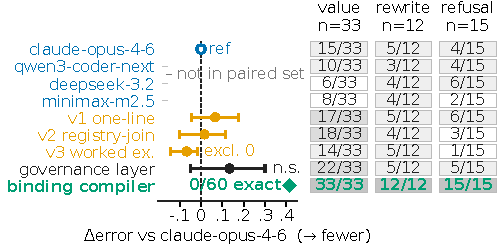
\includegraphics[width=\columnwidth]{fig3_paired_stratified.pdf}
\Description{Two panels sharing the row order of the main results table.
Left: per-arm paired error reduction against the pre-registered reference
backbone with cluster-bootstrap 95 percent intervals over nine databases;
the only interval excluding zero belongs to a prompt variant, in the wrong
direction, and the compiler's zero-error row is a deterministic transcript
drawn without an interval. Right: accuracy stratified by gold form (value,
rewrite, refusal) with the correct count over each form's denominator
printed in every cell.}
\caption{Effects with uncertainty (left: paired error reduction vs the
reference, cluster-bootstrap 95\% CIs over nine databases; only v3's excludes
zero, wrong-signed) and accuracy by gold form (right: the three denominators
partition the true denominator of 60), in the row order of
Table~\ref{tab:main}.}
\label{fig:taxonomy}
\end{figure}

\subsection{E1--E2: The Gap, and That One-Line Prompting Does Not Close It}
\label{sec:eval-gap}

\looseness=-1 The four plain baselines err on 60.0\%, 71.7\%, 73.3\% and 76.7\% of the
60 Chinese questions (Table~\ref{tab:main}): every family clears the pre-registered
floor (criterion A$'$, $\min\geq0.30$) by
$2\times$; every cluster interval excludes zero, too
wide to rank families. Figure~\ref{fig:taxonomy}'s stratified panel shows a
two-sided shape: on
the refusal side the baselines answer through 11, 11, 9 and 13 of the
15 refusals, refusing correctly on 4, 4, 6 and 2 --- no class
demanded; over the eight LLM arms the refusal classes
recover as $\OOV$ 4 of 32 chances, $\DBL$ 2 of 24, $\AM$ 15 of 40, $\MC$ 10
of 24. On
the value side the
errors are wrong values and failed
executions, not missing SQL (\texttt{deepseek-3.2} instead over-refuses 19
of 45; \texttt{minimax-m2.5} fails to execute on 24),
and they stack with resolution depth: \texttt{codebase\_community} --- the
deepest chain, carrying 8 of
the 18 policy rows --- is among the hardest
clusters for every arm, the baselines erring on $6,6,7,7$ of 7.

\smallskip\noindent\looseness=-1\textbf{Prompting does not close it.} The three variants
score 53.3\%, 58.3\% and 66.7\% against the backbone's 60.0\%: the best
removes 8 of the reference's 36 errors ($\mathrm{elim}=0.222$), the worst
removes 2 while adding 6, and all three
sit under the pre-registered C$'$ line for \emph{prompt} variants
($\max=0.222<0.40$). The refusal side barely moves (correct refusals
$4\to6,3,1$; answering through $11\to9,12,14$); the instruction-heavy variants
add wrong values and executions.

\subsection{E3: The Governance-Informed Arm}
\label{sec:eval-gov}

\looseness=-1 If the failure were an information gap, the governance layer would close it. One pre-registered arm on the reference backbone prepends, to the
variant-2 instruction, its database's \emph{entire} governance layer ---
all ten registries, all rows, both committed versions, serialised
deterministically and packaged per \emph{database} so no row can be selected
using the question (16{,}176--28{,}279-character prompts; no truncation
fired); packaging, rewrite rules and predictions were frozen before any call.
It bounds what a governed metric layer's
\emph{content}~\cite{semlayerbench} buys in context.

\smallskip\noindent\looseness=-1\textbf{Result.} The arm errs on $46.7\%$ ($28/60$), the
best LLM arm. It eliminates 13 of the reference's 36 errors and introduces 5
new ones (net $+8$; Figure~\ref{fig:taxonomy}, left panel); against
\texttt{trivial\_v2}, which isolates the
instruction, 11 fixed against 4 broken --- content, not instruction, carries
the gain, instruction alone moving one question ($36\to35$) against
content's
$35\to28$. The pre-registered three-case rule puts the arm in
case \emph{(iii)}: $\mathrm{elim}_{\mathrm{gov}}=13/36=0.361<0.40$, \emph{no
substantial elimination} --- the claim frozen before the run:
\textbf{under this protocol} (single turn, 512-token cap, database-level governance content plus
instruction), the frozen run does not substantially eliminate the
as-of gap; we do not extrapolate. Two post-registered restatements say how
firmly~\cite{asofgov-tr}: across five repetitions (rep\,1 the
frozen, scored one) elimination spans $0.361$--$0.417$, straddling the
$0.40$ line, and the paired nine-cluster 95\% CI for the
absolute error reduction is $[-0.05,0.30]$ --- ordering stable in all
five, magnitude unresolved at nine clusters. The frozen predictions were
optimistic --- all 8 observed error counts
exceed their point predictions and 7 of 8 exceed the 80\% interval's upper
end --- and the miss ledger is accounted item by item
in~\cite{asofgov-tr}, the elimination miss's frozen interval and the
denominator's own overshoot included.

\smallskip\noindent\looseness=-1\textbf{Where the residue sits is the finding.}
\emph{(a)}~On the seven refusal questions whose gold label is
\emph{provably} not registry-derivable --- \S\ref{sec:eval-setup}'s witness
pairs materialise both labels under identical content, so only a data probe
decides ($\OOV$ emptiness, $\MC$(ii) denominator mass, $\AM$(iv) realisation
difference) --- the arm errs on \textbf{6 of 7}, every one by answering.
\emph{(b)}~Where a registry line \emph{can} decide it errs on only \textbf{1 of
5} --- though
the two sets are not length-matched (means $24.6$k vs $20.3$k characters), so
this contrast inherits the dilution/depth entanglement below.
\emph{(c)}~On the three \texttt{DISCLOSURE-BLOCKED} questions it holds the
policy rows that block the answer --- and answers all three: \textbf{a
policy on file is not a policy enforced}. \emph{(d)}~On the eight
version-flip answers (\S\ref{sec:eval-mech}) it errs on 3 --- two by
resolving the wrong version--window pair, one a failed execution.
\emph{(e)}~The cluster gradient repeats it:
\texttt{codebase\_community} stays at 6/7 errors while shallow-chain clusters
nearly repair (\texttt{financial} $4\to1$ of 8, \texttt{debit} $3\to1$,
\texttt{world\_1} $2\to1$), while \texttt{card\_games} and
\texttt{european\_football\_2} each regress $2\to4$ --- the third- and
fourth-longest packages. Correct refusals move $4\to5$ of 15, over-refusal
is 1 of 45 --- \texttt{trivial\_v2}'s level, down from the plain backbone's
5. \emph{(f)}~The probe ceiling is measured:
crediting the arm with all six probe-decidable residuals --- four sit
among the reference's 36 errors, two its own regressions --- leaves
$22/60$, elimination at most $17/36=0.472$, past the $0.40$ line; an
execution loop recovers failed executions by construction, so
further crediting all nine execution-error residuals (disjoint from
the six; seven among the 36, two regressions) leaves $13/60$, at most
$24/36=0.667$: the verdict is a fact about probe-less, feedback-less
passes, and the four policy/registry
residuals are not probe-decidable at all.

\smallskip\noindent\looseness=-1\textbf{Three alternative explanations, checked.}
\emph{Context dilution}: package length is constant within a database
(spread ${\leq}80$ characters) and monotone in chain depth, so this design
cannot separate dilution from depth --- the question-level point-biserial is
$r=0.400$, but at the cluster unit it is $r=0.774$ ($t=3.24$,
$\mathrm{df}=7$), and \texttt{codebase} (28.3k) errs 6/7 against
\texttt{financial} (23.5k) at 1/8: we do not claim dilution excluded. \emph{Transport faults}: the arm had zero empty responses
--- excluded. \emph{Imperative compliance} (obeying a cross-window
imperative instead of judging it): both $\AM$(ii) imperatives are correctly
refused --- excluded as the driver.

\smallskip\noindent\looseness=-1\textbf{Non-degeneracy, adversarially confirmed
(ND-4).} This arm is the designed attack on our own benchmark: on the
retired public track, whose registries carried expressions and coverage
literals, the same protocol scored $0/20$ --- a lookup, not a finding. Handed strictly
more content, it errs \emph{where} the design predicts.

\subsection{E4: The Certified Compiler}
\label{sec:eval-mech}

\looseness=-1 The compiler decides all 60 in agreement with the frozen gold --- values,
refusal classes \emph{and subtypes}, rewrite kinds --- emitting 33
answers, 12 rewrites and 15 refusals (Table~\ref{tab:suite}); the refusals
coincide with the 15 the specification declares unanswerable --- 12 by the
binding semantics of \S\ref{sec:semantics}, 3 by the disclosure layer of
\S\ref{sec:rewrite} --- so the refused
share 0.25 is not caution, and re-emission is byte-stable. The
$0\%$ is a \emph{constructive upper bound}: the registered binding rules are
implementable and cover these 60 questions --- not that a learned system
generalises. The compiler consumes the structured intent $\sigma$ of
Definition~\ref{def:query}; the LLM arms read the same declarations from the
question's natural language (parsing language into $\sigma$ is out of
scope).

\smallskip\noindent\looseness=-1\textbf{The disclosure layer, exercised.} This suite makes \S\ref{sec:rewrite} earn its place on gold: three
\texttt{DISCLOSURE-BLOCKED} refusals where the masked, $k$-gated ladder has
no legal point; five
granularity roll-ups, one whose $k$ moves $10\to20$ \emph{between versions}
(the same
question answers under $v1$, rewrites under $v2$); and two mask degradations
whose transform compiles into the emitted SQL --- each closed by the
independent verifier (\S\ref{sec:eval-cert}), not by our own replay. Ablating the rewrite stage
is arithmetic rather than a run: refusing wherever the request is not
directly bindable turns the 12 rewrites into refusals, the refused share
$0.25\to0.45$, the error rate $0\%\to20.0\%$, every gold refusal
class unchanged --- the binding layer, not the search, carries the classes.

\smallskip\noindent\looseness=-1\textbf{The version axis, exercised.} Four question
pairs pin one question at two declared times so the answer \emph{flips}
with the in-effect version; the sharpest is real history ---
Formula~1's 2009 vs.\ 2010 points schemes value the same 2009 season at
$100.0$ vs.\ $252.0$ --- alongside a problem-loan caliber change
($0.1368\to0.0855$) and two further re-scopings.
One question reads \emph{off-diagonal}, pinning $v1$ under
$\ver(T)=v2$: legal exactly because the certificate carries the explicit
commitment marker, whose deletion is one forgery below.

\subsection{E5: Certificates and Forgeries}
\label{sec:eval-cert}

\looseness=-1 The independent verifier accepts $60/60$ certificates; the
discriminating experiment is forgery: 78 forged certificates in all --- 34
pre-registered with the suite over \emph{11 unmodified compiler certificates
as bases} (all 11 accept), 44 post-registered with the V6a+ hardening below.
The verifier rejects $34/34$, each on the check its construction
pre-registered: 6 value/window lies (one an empty-denominator refusal flipped
to an answer, caught by \emph{re-executing} the probe); 5 \emph{field
deletions} --- $\nu,\alpha,\rho,\delta$, refusal witness --- one per field, the
converse half of Proposition~\ref{prop:nonredundant}; 9 semantic lies; 10
disclosure forgeries (banned grain, \texttt{SELECT 999} for a support
transcript, masks dropped); and 4 refusal-class substitutions. \emph{One
boundary case is accepted and we say so}: deleting \emph{part} of a refusal's
blocking-policy list (still non-empty and registered) passes --- beyond
non-emptiness that list is not load-bearing.

\smallskip\noindent\looseness=-1\textbf{Hardened after external review
(V6a+).} An external review (2026-08) exhibited what this battery had not
probed: V6a accepted wrong-aggregate, swapped-leg, constant-output and
narrowed-window mutations of a genuine certificate. V6a+ responds, scope
frozen first~\cite{asofgov-tr}: the 5 reproduction mutations
reject as pinned regressions, each on its pinned reason code; five new
families over 22 accepted bases --- F6 wrong aggregate (6), F7 leg swap
(5), F8 wrong/absent predicate (8), F9 narrowed/widened
window (6), F10 constant/multi-row (6) --- reject $31/31$; the 34 keep every
frozen \emph{rejected-by} attribution, all 60 genuine still accept with
per-question verdicts identical. All four frozen predictions held.

\smallskip\noindent\looseness=-1\textbf{Round 2: outer-filter closure.} A
second external review (2026-08) exhibited a genuine ratio whose outer
\texttt{WHERE}, filtering the scalar answer to zero rows, V6a+ accepted --- now
rejected structurally and by an executed-arity check
(\S\ref{sec:cert:verifier}), the two exploits pinned. A new F11
outer-row-filter (8) rejects $8/8$; the family total is $78/78$ rejected,
$80/80$ with the pins~\cite{asofgov-tr}.

\smallskip\noindent\looseness=-1\textbf{Independence, measured.} A window
read off the shared question would restate what
the certificate committed to, so each role window is re-derived from
the registered as-of conventions over $(G_v,D)$: the verifier derives 50 of
60 windows itself and, under a strict switch refusing every presented
window, accepts exactly those $50/60$ --- the 10 rejections are the
8 questions whose window arrives as an explicit range request plus the
2 cross-window imperatives, where the presented coordinates \emph{are} the
declared input and the verifier fails closed.

% ---------------------------------------------------------------------
%  Table F-C -- D1-D15 divergence ledger.  GENERATED FILE, DO NOT EDIT.
%  Regenerate:  python3 tools/gen_table_divergence.py
%  Source of record: impl/INTEGRATION_REPORT.md section 5 (15-row table)
%  and section 2 (per-family check labels).  tools/gen_table_divergence.py
%  parses that table, asserts 15 rows / 5+5+5 / the 25-rejection family
%  decomposition, and fails rather than print stale content.
%  The last column's headline case is MEASURED, not asserted: see the
%  A/B recipe in the generator's module docstring.
%  Macros used (\MC, \beta_v ...) are \providecommand'd in 03-semantics.
% ---------------------------------------------------------------------
\begin{table}[t]
\centering
\scriptsize
\setlength{\tabcolsep}{2.0pt}
\renewcommand{\arraystretch}{0.93}
\caption{Every disagreement the two implementations had on their first
cross-check. \emph{Provenance}: this ledger was recorded during the two
sides' integration on the production (enterprise) track that motivated this
work, before the public suite of \S\ref{sec:eval-setup} existed; it is
specification-level content --- readings, checks, guard order --- and
carries no production data value, so it is reported as evidence about the
\emph{design}, not about the released benchmark.
\emph{Cls}: S~spec-reading, D~defect (subscript: which side),
R~registration gap; \emph{Right}: the side the frozen text vindicated;
\emph{Check}: the check that fired ($\dagger$~crashed). The 25 first-round
rejections were V0$\times9$, V6a$\times9$, V3$\times3$, V6b$\times2$,
V6c$\times1$, V4/V6c$\times1$, many-to-many onto these 15.
\emph{Value gold?}: would the integration suite's value-level gold --- 51
questions, 37 numeric and 14 refusal-token comparisons --- have failed? On
no row, and the cell says why not:
the value is unchanged; the lie is confined to the \emph{cert}ificate or
registry that gold never reads; the erring side is the \emph{verif}ier that gold
never runs; or the gold \emph{label} is itself what settled the reading. Both
readings per row:~\cite{asofgov-tr}.}
\label{tab:divergence}
\begin{tabular}{@{}lccll@{}}
\toprule
Divergence & Cls & Right & Check & Value\\
 & & & fired & gold?\\
\midrule
$D_{1}$ coverage domain gates before $\MC$? & S & spec & V6b & \ding{55}\,label\\
$D_{2}$ $\beta_v$ defined when both legs are NULL? & S & spec & V6b & \ding{55}\,verif.\\
$D_{3}$ prescribed anchor of an atomic metric & R & verif. & V0 & \ding{55}\,cert\\
$D_{4}$ must a ratio carry a caliber route? & R & verif. & V4, V6c & \ding{55}\,cert\\
$D_{5}$ is \texttt{avg\_handle\_hours} a ratio? & R & spec & V3 & \ding{55}\,label\\
$D_{6}$ must a rewrite emit $w^*$'s lower bound? & D$_{\mathrm{c}}$ & verif. & V6a & \ding{55}\,value\\
$D_{7}$ may an atom borrow another's binding row? & D$_{\mathrm{c}}$ & verif. & V3 & \ding{55}\,cert\\
$D_{8}$ probe bound: arithmetic or literal window & D$_{\mathrm{c}}$ & verif. & V6b & \ding{55}\,cert\\
$D_{9}$ does a month marker denote the month? & S & comp. & V6c & \ding{55}\,verif.\\
$D_{10}$ is a derived-table alias a read object? & D$_{\mathrm{v}}$ & comp. & V6a & \ding{55}\,verif.\\
$D_{11}$ does a conformed-dim join leave closure? & R & verif. & V6a & \ding{55}\,cert\\
$D_{12}$ replay of the interval-anchor predicate & D$_{\mathrm{v}}$ & comp. & V6a$^{\dagger}$ & \ding{55}\,verif.\\
$D_{13}$ where the re-anchoring $\bar a$ is carried & S & spec & V0 & \ding{55}\,cert\\
$D_{14}$ how a delta question presents $\vec\omega$ & R & spec & V0 & \ding{55}\,cert\\
$D_{15}$ certificate spelling of an unreg. anchor & S & either & V0 (V2) & \ding{55}\,cert\\
\midrule
\multicolumn{4}{@{}l}{5 S $\cdot$ 3+2 D $\cdot$ 5 R\ \ (25 rejections $\to$ 15 causes)} & \ding{55}\,$0/15$\\
\bottomrule
\end{tabular}
\end{table}


\subsection{E6: What Independence Bought}
\label{sec:eval-divergence}

\looseness=-1 The first cross-check of the two implementations --- recorded during their
integration on the production track that motivated this work
(Table~\ref{tab:divergence}) ---
\emph{rejected 25 of the 51 certificates then in force}, resolving into 15
distinct root causes: 5 implementation defects (3 compiler-side, 2
verifier-side), 5 registration gaps, 5 specification-reading divergences. Not
one would have been caught by checking values against gold --- the three
compiler-side defects each returned the right answer under a
non-re-derivable certificate claim. Two lessons shaped the public base: in
every registration gap the load-bearing content lived in a free-text note or
compiler source ---
\emph{certificate checkability is a measurable proxy for governance
registration completeness}, enforced as \S\ref{sec:eval-setup}'s seed
discipline --- and three of the five specification
divergences sit on when a guard's subject is undefined, each moving a
refusal \emph{class}; this suite's frozen guard-order adjudications
descend from those rows.

\subsection{Cost, and Threats to Validity}
\label{sec:eval-cost}
\label{sec:eval-threats}

\noindent\looseness=-1\textbf{What certification costs.} Counting work only (warm
process, connections held; all timings on a 10-core arm64 macOS 15
machine; Python 3.9.6, DuckDB 1.4.4), verifying a decision costs a median
$17.7\times$ the answering query it certifies --- $17.0$\,ms against
$1.31$\,ms, per-question paired ratios over the 45 questions that emit SQL
(the marginal medians' own quotient is $12.9\times$), spanning $2.5\times$ to
$44.4\times$ (p90 $36.1\times$); none is cheaper to verify than to answer, and
the certificate is a paired median $10.2\times$ the query's bytes
(pretty-printed; $8.4\times$ minified), the tail
being coverage replay on the largest governed tables ($0.18$\,s warm). The 60
per-certificate cold
medians (median of 5 processes per certificate) sum to $7.60$\,s ---
median 116\,ms, p90 144\,ms, max 288\,ms, 53\,ms of it process floor; as whole
cold processes the paired median falls to $1.8\times$, the fixed per-process
cost dominating. \S\ref{sec:rewrite}'s probe bound (\cite{asofgov-tr}) covers the
in-window probe term; the full-scan class it exempts has \emph{no} instance
here ($\AM$(iv) audits are window-bounded), so we exhibit no
scan-amplification regime and report no scalability sweep.

\smallskip\noindent\looseness=-1\textbf{Threats.} \emph{Sixty questions is the unit
count, not the evidence mass}: each unit is a governed instance carrying
executed gold, a verifier-accepted certificate and an eight-arm response
grid; leave-one-cluster-out moves no ordering:
every fold keeps each plain baseline's error ${\geq}0.40$, governance below
all four, the compiler at
$0$~\cite{asofgov-tr}. \emph{One sample per question is the protocol}: five
reps of both headline arms (rep\,1 the frozen run) hold the ordering in all
five, flips ${\leq}13.3\%$ per
arm~\cite{asofgov-tr}. \emph{Nor does governance-blind temporal-SQL close
it}: post-registered hand-built arms err $28/60$ same-window --- level
with the governance-informed arm; $23/60$ crediting five bare
\texttt{NULL}s as refusals --- $54/60$ all-history, values $6/33$ under
both readings~\cite{asofgov-tr}. \emph{Authored governance over real
data}: the fact rows are shipped public data save \texttt{world\_1}'s
authored history, but the layer over them is ours; the mitigations are
structural (non-degeneracy gates, witness pairs, distractor density, leak
audit) and total transparency, not independence of authorship.
\emph{Scoring concessions run toward the baselines}: LLM refusals need no
class, rewrites no declaration, a multiset amnesty admits shape-degenerate
answers, and on the five hull-trim questions a window-blind aggregate equals
gold by construction --- the form split in Table~\ref{tab:taxonomy} keeps the
headline from hiding there (value errors 11/33
even with those freebies); and on one of the four version-flip pairs
(\texttt{california\_schools}) the two gold values differ by $0.48\%$, inside
the $0.5\%$ scoring tolerance, so that pair credits a version-blind answer.
Running the other way, the compiler is handed the $\sigma$ the LLM arms must
recover from text (\S\ref{sec:eval-mech}); a post-registered arm that
extracts $\sigma$ from the question text and hands it to the compiler errs
$5/60$~\cite{asofgov-tr} --- recovering $\sigma$ is not where the difficulty
lives.
\emph{One backbone} carries the variant and governance arms --- conclusions
about \texttt{claude-opus-4-6}; cross-family columns carry
\S\ref{sec:eval-setup}'s gateway caveat. \emph{The protocol is
cross-lingual} (\S\ref{sec:eval-setup}): the three Chinese-native families
still err more than the backbone ($71.7/73.3/76.7$ against $60.0$ ---
gateway-confounded columns, intervals too wide to rank families); a
post-registered English run of both headline arms moves each arm one
question ($35/60$, $29/60$ against $36/60$, $28/60$), ordering and
probe-side concentration intact~\cite{asofgov-tr}: language does not drive
the gap. \emph{The
governance-informed comparator is bounded in our favour}
(\S\ref{sec:eval-gov}): full-layer packaging is an upper bound on what
in-context governance buys, not a tuned opponent's floor; \emph{prediction misses are published} (\S\ref{sec:eval-gov}).
\emph{What no arm has} is
\emph{execution feedback}: every system answers from one statement --- one
pass cannot run the probes that decide the hard classes --- and \emph{prompt
technique is one line deep} --- no decomposition, self-consistency, in-domain
few-shot or multi-turn arm.

% =====================================================================
% Section 9 -- RELATED WORK   (target: ~0.75 page incl. Table 5)
% The four-nearest-neighbour delineation is a RED LINE: it is carried by
% Table~\ref{tab:delta} plus one dense paragraph, one sentence per
% neighbour ("what it does / which requirement it lacks").  The temporal
% database and NL2SQL lineages get one sentence each; refusal, disclosure
% rewriting and certificates are folded into a single closing paragraph.
% (2026-08-24, author decision) The concurrent-submission paragraph and the
% substrate row/citations were removed; the remaining citation keys of the
% long version are retained.
% =====================================================================

\section{RELATED WORK}
\label{sec:related}

\begin{table}[t]
\centering
\footnotesize
\setlength{\tabcolsep}{2.6pt}
\renewcommand{\arraystretch}{0.95}
\caption{The four nearest neighbours and the closest temporal-database
lineage, against the four properties
as-of correctness needs: none binds a
question to a point on both axes, none makes a refusal a checkable value.}
\label{tab:delta}
\begin{tabular}{@{}lcccc@{}}
\toprule
& versioned & valid-time & typed & checkable\\
& sem.\ layer & as-of bind & refusal & certificate\\
\midrule
schema-evolution robustness~\cite{evoschema}      & $\circ$ & --      & --      & --\\
bitemporal agent memory~\cite{memstrata}          & --      & \checkmark & --   & --\\
lakehouse time travel~\cite{deltalake,iceberg}    & --      & $\circ$ & --      & --\\
transaction time + schema evol.~\cite{primatt,prism} & $\circ$ & \checkmark & -- & --\\
static semantic layers~\cite{semlayerbench}       & --      & --      & --      & --\\
\midrule
\textbf{this paper}                               & \checkmark & \checkmark & \checkmark & \checkmark\\
\bottomrule
\end{tabular}
\par\smallskip
{\scriptsize\raggedright $\circ$ = partial: schema versions, not a governance
layer; snapshot-level time travel without a semantic layer.\par}
\end{table}

\noindent\looseness=-1\textbf{The four nearest neighbours} each hold one half of the problem
(Table~\ref{tab:delta}).
\emph{Schema-evolution robustness}: EvoSchema~\cite{evoschema} perturbs schemas
but asks a model to be \emph{insensitive} to the version it faces; as-of
correctness asks it to be \emph{bound} to a declared one, saying so when no
binding exists. \emph{Bitemporal agent memory}: MemStrata~\cite{memstrata} keeps
\texttt{valid\_from}/\texttt{valid\_to}, supersession and as-of retrieval, but
over retrieved facts, not compiled queries: no metric semantics, no
compile-time decision. \emph{Lakehouse time travel}: snapshot
pins~\cite{deltalake,iceberg} are a genuine as-of capability we consume, but
answer ``which bytes'', not ``which meaning'', and return a number exactly
where we refuse. \emph{Static semantic layers}: a governed metric layer measurably
improves LLM analytics accuracy~\cite{semlayerbench} --- our nearest
neighbour and a natural baseline, whose in-context content
\S\ref{sec:eval-gov} bounds --- but a static document without versions,
as-of binding or refusal. Substrates that own the version transition and
disclaim metric correctness leave exactly the space this paper
occupies; Theorem~\ref{thm:degen} makes the relationship precise.

\smallskip\noindent\looseness=-1\textbf{Lineages we inherit.} Temporal databases give us the
data axis wholesale --- valid and transaction time and the languages over
them~\cite{tquel,tsql2,tempmod,tempalign,sql2011,timelineindex}, querying under
schema evolution~\cite{primatt,prism}, dataset and relational
versioning~\cite{dsversioning,orpheusdb,decibel} --- but no second axis for a
\emph{governance} layer, no typed value for inability to answer --- so a hand-built
temporal-SQL implementation of the sixty queries is a point in the compiler's
design space minus the refusal classes and the certificate. Post-registered, we
built one~\cite{asofgov-tr}: it errs $28/60$ --- level with the
governance-informed arm --- all 15 refusals answered ($23/60$ crediting its
five bare \texttt{NULL}s); an all-history twin errs $54/60$; values
$6/33$ --- the data axis is not the bottleneck. The NL2SQL lineage~\cite{seq2sql,ratsql,spider,bird,dinsql,dailsql,
nl2sqlsurvey,nl2sqltoday,solvednot} treats the database as a fixed
target --- our evidence base takes nine of its databases~\cite{spider,bird}
and registers the governance layer binding needs; time-sensitive
QA~\cite{tdbench} scores answers, not queries.

\smallskip\noindent\looseness=-1\textbf{Refusal, disclosure, certificates.} Refusal is studied
as completeness over incomplete data~\cite{completeness} and abstention on
unanswerable questions~\cite{ehrsql}; ours are decidable predicates over the
governance state (Proposition~\ref{prop:decidable}) carrying a class and a
replayable witness. Fine-grained access control~\cite{finegrained},
purpose-limited disclosure~\cite{hippocratic} and anonymity
thresholds~\cite{kanon,ldiversity} are long-standing, our grain and mask
lattices ordinary instances; \S\ref{sec:rewrite} adds the joint statement
\emph{after} temporal binding. Certifying
algorithms~\cite{certifying}, provenance~\cite{semirings,provsurvey} and
authenticated query processing~\cite{authindex,vsql} are our certificates'
tradition; we add the coordinates they assume fixed and a certificate for
a \emph{refusal}, which none can express.

% =====================================================================
% Section 10 -- CONCLUSION, LIMITATIONS, AVAILABILITY, AI DISCLOSURE
% (target: ~0.5 page).  The three closing/mandatory blocks are merged into
% one section; the generative-AI disclosure keeps its full wording.
% Every limitation named here is also stated where the claim is made.
% PILOT2 MIGRATION (2026-08-04): all numbers on the public 60-question
% base; the version-axis "never exercised" caveat is retired (it is
% exercised now) and replaced by the three genuinely unexercised defence
% paths; the artifact inventory matches the released public base.
% =====================================================================

% Title shortened 2026-08-06 (page ceiling): the two-line heading cost a
% wrapped line; limitations keep their bold paragraph labels below.
\section{CONCLUSION AND AVAILABILITY}
\label{sec:concl}

\noindent\looseness=-1\textbf{Conclusion.} As-of correctness for governed analytical queries
is a compile-time binding problem (compile-time relative to the model: the
compiler decides by running probes against the store): we gave it a
bi-temporal semantics whose refusals are values, a decidable four-way
classification --- under disclosure, a maximal legal rewrite or a complete
structured refusal --- and certificates an independent verifier re-derives
from the governance tables and data. On a fully public base of 60 Chinese
questions four frontier model families err on 60.0--76.7\%, no prompt variant (53.3--66.7\%)
crosses the pre-registered elimination line, and the entire governance layer in
context still leaves 46.7\%, its refusal-side residue on decisions that need a
data probe: under this protocol --- one statement per question, no execution
feedback --- in-context governance yields no substantial elimination. Three findings carry forward:
binding is an \emph{execution-time} property no prompt content substituted
for under this protocol --- the informed model executed
a disclosure policy on file zero times in three; disagreement between the two implementations was as often
\emph{registrational} as implementational --- checkability measures how
much of a layer is really governed; and the
disagreements surviving the specification move refusal \emph{classes} ---
the price of making refusal a first-class value.

\smallskip\noindent\looseness=-1\textbf{What we did not prove.} Answer soundness
(Theorem~\ref{thm:certsound}(b)) rests on the still-open ``syntax
implies semantics'' assumption (A-tmpl) over Definition~\ref{def:tmpl}'s
class, Theorem~\ref{thm:sound}(a) on its \emph{(A-emit)} bridge; the
checking relation verifies a rewrite legal and
its cut trace consistent, \emph{not} maximal; continuous time,
window bargaining, lag rules and the full maximal frontier are out of
scope by~(A6). The version axis is now exercised (two committed versions per
database, four flip pairs, one off-diagonal pin), but three defence paths
have no gold instance (refusal before the first
governance commit, an uncommitted version pin, the certificate side of an
alias-missing $\MC$(i)), and one adjudication is unresolved: whether a
delta-period window needing a hull trim rewrites or refuses.

\smallskip\noindent\looseness=-1\textbf{What the numbers license} (\S\ref{sec:eval-threats}).
The $0\%$ is a constructive upper bound over this suite --- nothing
follows about unseen questions or free-form language --- and the $46.7\%$
set against it bounds what in-context governance buys from a single
statement; no execution-capable (agentic) arm was run --- the probe-oracle
ceiling (\S\ref{sec:eval-gov}), execution-error residuals credited,
bounds the recoverable share at $0.667$.

\smallskip\noindent\looseness=-1\textbf{Artifact availability.} Everything needed to
reproduce every number is at
% (A1) The URL below expands \artifacturl, defined once in main.tex.  Do
% not hard-code a literal URL here -- edit the macro.  The repository is
% real; the stale "placeholder" footnote was dropped 2026-08-04 once the
% locator was filled (the make-it-public click remains the author item).
\url{\artifacturl}: compiler and
independent verifier with the CI import-disjointness check; the nine
warehouses with registries, per-row real/authored provenance and gold SQL;
the 60 questions with gold values, refusal classes/subtypes, rewrite kinds
and frozen scoring; the non-degeneracy gate reports; the arms
pre-registration with predictions and both freeze manifests; the raw response cache for all $8\times60$ pairs \emph{and} the voided
\texttt{trivial\_v2} first run; the 60 certificate envelopes, the forgery
generator with its 11 bases and 34 forgeries, the cost measurements and the
cluster-bootstrap script with its frozen seed; one driver re-runs the
offline pipeline, the frozen cache reproducing every number without an
API key. Not released: the enterprise development seeds --- their only
exhibits are \S\ref{sec:intro}'s motivating rates and
Table~\ref{tab:divergence}'s ledger, provenance-marked in place; no
public-suite number depends on them.

\smallskip\noindent\looseness=-1\textbf{Disclosure of generative AI use.} In accordance with
the PVLDB and ACM publication policies on generative-AI tools, we disclose that
large language models were used throughout the production of this work: in
drafting and revising definitions, theorems and proof sketches; in
implementing the compiler, verifier, forgery generators and figure pipeline;
in building and running the evaluation harness; and in drafting and editing
this manuscript. Large language models are also the
object of study in \S\ref{sec:eval}, as evaluated systems. All definitions, theorems, proofs, experimental protocols, numbers and
claims were reviewed and are vouched for by the authors, who take full
responsibility for the entire content of this paper, including any errors.

% Acknowledgements are a camera-ready item and are omitted here to stay inside
% the 12-page body limit; restore the block below before the final version.
% \begin{acks}
% ...
% \end{acks}


% =====================================================================
%  MANDATORY BLOCKS (Vol.20).  The PVLDB Reference Format block, the
%  CC BY-NC-ND 4.0 licence footnote and the PVLDB Artifact Availability
%  block are all emitted by \vldbtopmatter above (pvldb.sty) -- they must
%  not be reproduced by hand.  The generative-AI disclosure and the prose
%  availability statement live in Section~\ref{sec:concl}; both count
%  against the 12-page body limit.
% =====================================================================

\balance
\bibliographystyle{ACM-Reference-Format}
\bibliography{refs}

\end{document}
